\chapter{在Direct3D中绘制(Drawing in Direct3D)}
\begin{flushleft}
在前一章中,我们主要关注渲染管线的概念和数学方面。 本章反过来关注配置渲染管道,定义顶点和像素着色器以及将几何图形提交到渲染管道进行绘制所需的Direct3D API接口和方法。 到本章结束时,您将能够绘制出具有纯色的3D框或线框模式。\\
~\\
{\large Objectives:}
\begin{itemize}
    \item 发现用于定义,存储和绘制几何数据的Direct3D接口方法。
    \item 学习如何写一个基本顶点和像素着色器
    \item 了解如何用管线状态对象配置渲染管线
    \item 理解如何创建和绑定缓冲数据常量到管线中,并且熟悉根签名
\end{itemize}
\end{flushleft}
\section{顶点和顶点布局(Vertices and Input Layouts)}
\begin{flushleft}
5.5.1节已经讲过,在Direct3D中,顶点由空间位置和各种附加属性组成,Direct3D可以让我们灵活地建立属于我们自己的顶点格式;换句话说,它允许我们定义顶点的分量。要创建一个自定义的顶点格式,我们必须先创建一个包含顶点数据的结构体。例如,下面是两种不同类型的顶点格式;一个由位置和颜色组成,另一个由位置、法线和纹理坐标组成。
\end{flushleft}
\begin{lstlisting}
struct Vertex1
{
    XMFLOAT3 Pos;
    XMFLOAT4 Color;
}
struct Vertex2
{
    XMFLOAT3 Pos;
    XMFLOAT3 Normal;
    XMFLOAT2 Tex0;
    XMFLOAT2 Tex1;
}
\end{lstlisting}
\begin{flushleft}
我们定义好顶点构造体后,需要对该定点构造体进行描述然后提供给 Direct3D,让它知道如何去处理每个分量。此描述以D3D12\_INPUT\_LAYOUT\_DESC结构表示的输入布局描述(input layout description)的形式提供给Direct3D:
\begin{lstlisting}
typedef struct D3D12_INPUT_LAYOUT_DESC
{
    const D3D12_INPUT_ELEMENT_DESC *pInputElementDescs;
    UINT NumElements;
} D3D12_INPUT_LAYOUT_DESC;
\end{lstlisting}
一个输入布局描述就是一个简单的 D3D12\_INPUT\_ELEMENT\_DESC 元素数组和元素的数量。\\
~\\
D3D12\_INPUT\_ELEMENT\_DESC数组中的每个元素描述了对应的顶点结构体的分量。如果顶点构造体有两个分量,则对应的 D3D12\_INPUT\_ELEMENT\_DESC数组就有2个元素。D3D12\_INPUT\_ELEMENT\_DESC 定义如下:
\begin{lstlisting}
typedef struct D3D12_INPUT_ELEMENT_DESC
{
    LPCSTR SemanticName;
    UINT SemanticIndex;
    DXGI_FORMAT Format;
    UINT InputSlot;
    UINT AlignedByteOffset;
    D3D12_INPUT_CLASSIFICATION InputSlotClass;
    UINT InstanceDataStepRate;
} D3D12_INPUT_ELEMENT_DESC;
\end{lstlisting}
1. SemanticName: 一个与元素相关的字符串。它可以是任何有效的语义名。语义(semantic)用于将顶点结构体中的元素映射为顶点着色器参数(参见图\ref{fig:6-1})。\\
\begin{figure}[h]
    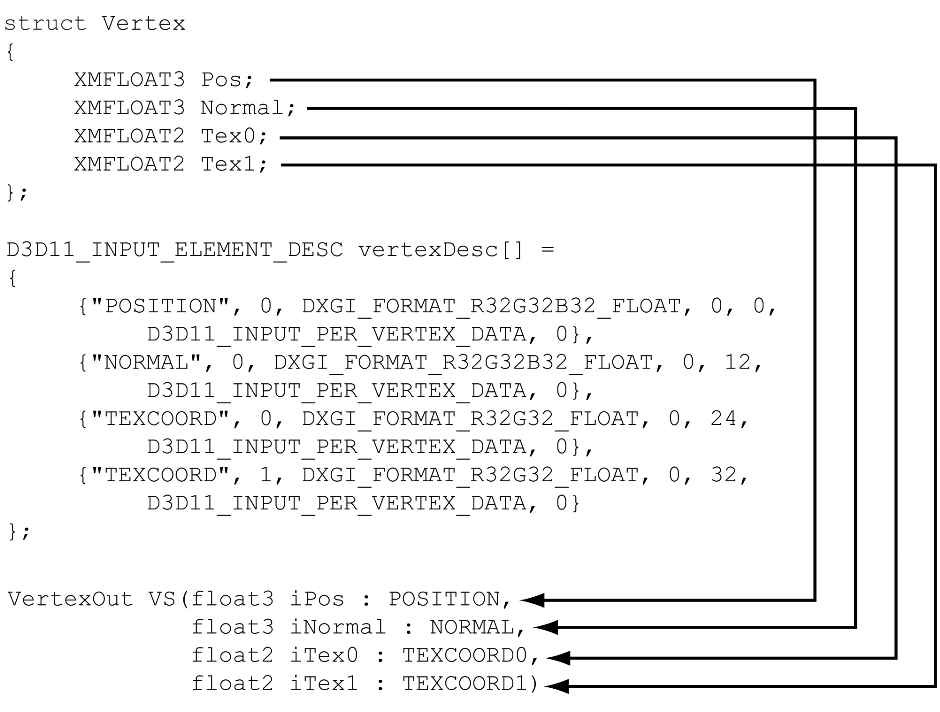
\includegraphics[width=\textwidth]{6-1}
    \centering
    \caption{顶点结构体中的每个元素分别由D3D11\_INPUT\_ELEMENT\_DESC数组中的对应元素描述。语义名和语义索引提供了一种将顶点元素映射为顶点着色器参数的方法。}
    \label{fig:6-1}
\end{figure}
2. SemanticIndex:附加在语义上的索引值。图\ref{fig:6-1}说明了使用该索引的原因;举例来说,当顶点结构体包含多组纹理坐标时,我们不是添加一个新的语义名,而是在语义名的后面加上一个索引值。在着色器代码中没有指定索引的语义默认索引为0,例如,在图\ref{fig:6-1}中的POSITION相当于POSITION0。\\
3. Format:一个用于指定元素格式的DXGI\_FORMAT枚举类型成员;下面是一些常用的格式:
\begin{lstlisting}
DXGI_FORMAT_R32_FLOAT          // 1D 32-bit float scalar
DXGI_FORMAT_R32G32_FLOAT       // 2D 32-bit float vector
DXGI_FORMAT_R32G32B32_FLOAT    // 3D 32-bit float vector
DXGI_FORMAT_R32G32B32A32_FLOAT // 4D 32-bit float vector
DXGI_FORMAT_R8_UINT            // 1D 8-bit unsigned integer scalar
DXGI_FORMAT_R16G16_SINT        // 2D 16-bit signed integer vector
DXGI_FORMAT_R32G32B32_UINT     // 3D 32-bit unsigned integer vector
DXGI_FORMAT_R8G8B8A8_SINT      // 4D 8-bit signed integer vector
DXGI_FORMAT_R8G8B8A8_UINT      // 4D 8-bit unsigned integer vector
\end{lstlisting}
4. InputSlot:指定当前元素来自于哪个输入槽(input slot)。Direct3D支持16个输入槽(索引依次为 0到15),通过这些输入槽我们可以向Direct3D传入顶点数据。例如,当一个顶点由位置元素和颜色元素组成时,我们既可以使用一个输入槽传送两种元素,也可以将两种元素分开,使用第一个输入槽传送顶点元素,使用第二个输入槽传送颜色元素。Direct3D可以将来自于不同输入槽的元素重新组合为顶点。在本书中,我们只使用一个输入槽,但是在本章结尾的练习2中我们会引导读者做一个使用两个输入槽的练习。\\
5. AlignedByteOffset:对于单个输入槽来说,该参数表示从顶点结构体的起始位置到顶点元素的起始位置之间的字节偏移量。例如在下面的顶点结构体中,元素Pos的字节偏移量为0,因为它的起始位置与顶点结构体的起始位置相同;元素Normal的字节偏移量为12,因为必须跳过由Pos占用的字节才能到达Normal的起始位置;元素Tex0的字节偏移量为24,因为必须跳过由Pos和Normal占用的字节才能到达Tex0的起始位置;元素Tex1的字节偏移量为32,因为必须跳过由Pos,Normal和Tex0占用的字节才能到达Tex1的起始位置。\\
\begin{lstlisting}
struct Vertex2
{
    XMFLOAT3 Pos;     // 0-byte offset
    XMFLOAT3 Normal;  // 12-byte offset
    XMFLOAT2 Tex0;    // 24-byte offset
    XMFLOAT2 Tex1;    // 32-byte offset
}
\end{lstlisting}
6. InputSlotClass:目前指定为D3D12\_INPUT\_PER\_VERTEX\_DATA;其他选项用于高级实例技术。\\
7. InstanceDataStepRate:目前指定为0;其他值只用于高级实例技术。\\
~\\
对于前面的两个示例顶点结构体Vertex1和Vertex2来说,对应的输入布局描述为:
\begin{lstlisting}
D3D12_INPUT_ELEMENT_DESC desc1[] = 
{
    {"POSITION", 0, DXGI_FORMAT_R32G32B32_FLOAT, 0, 0, 
                 D3D12_INPUT_PRE_VERTEX_DATA, 0},
    {"COLOR",    0, DXGI_FORMAT_R32G32B32A32_FLOAT, 0, 12, 
                 D3D12_INPUT_PRE_VERTEX_DATA, 0}
};
D3D12_INPUT_ELEMENT_DESC desc2[] =
{
    {"POSITION", 0, DXGI_FORMAT_R32G32B32_FLOAT, 0, 0,  
                 D3D12_INPUT_PRE_VERTEX_DATA, 0},
    {"NORMAL",   0, DXGI_FORMAT_R32G32B32_FLOAT, 0, 12, 
                 D3D12_INPUT_PRE_VERTEX_DATA, 0},
    {"TEXCOORD", 0, DXGI_FORMAT_R32G32_FLOAT, 0, 24, 
                 D3D12_INPUT_PRE_VERTEX_DATA, 0},
    {"TEXCOORD", 1, DXGI_FORMAT_R32G32_FLOAT, 0, 32, 
                 D3D12_INPUT_PRE_VERTEX_DATA, 0}
};
\end{lstlisting}
\end{flushleft}
\section{顶点缓冲(Vertex Buffers)}
\begin{flushleft}
为了让GPU访问顶点数组,我们必须把它放置在一个称为缓冲(buffer)的GPU资源容器中, 我们称存储顶点的缓冲区叫顶点缓冲区。 缓冲区比纹理资源简单; 它们不是多维的,并且没有mipmap,过滤器或多采样支持。 无论何时我们需要为GPU提供一系列数据元素(如顶点),我们都会使用缓冲区。\\
~\\
就像4.3.8节一样,我们通过填充一个 D3D12\_RESOURCE\_DESC结构体来创建一个 ID3D12Resource 对象,并将其作为缓冲区资源。然后调用 ID3D12Device::CreateCommitedResource 方法。D3D12\_RESOURCE\_DESC 成员详情见 4.3.8 节。Direct3D 12 提供一个 C++ 包装类 CD3DX12\_RESOURCE\_DESC,它是 D3D12\_RESOURCE\_DESC 的衍生类,提供了方便的构造函数和方法。特别是,它提供了以下方法来简化描述缓冲区的D3D12\_RESOURCE\_DESC的构造:
\begin{lstlisting}
static inline CD3DX12_RESOURCE_DESC Buffer(
    UINT64 width, 
    D3D12_RESOURCE_FLAGS flags = D3D12_RESOURCE_FLAG_NONE,
    UINT64 alignment = 0)
{
    return CD3DX12_RESOURCE_DESC(D3D12_RESOURCE_DIMENSION_BUFFER, 
            alignment, width, 1, 1, 1, 
            DXGI_FORMAT_UNKNOWN, 1, 0,
            D3D12_TEXTURE_LAYOUT_ROW_MAJOR, flags);
}
\end{lstlisting}
对于一个缓冲区,width 相当于缓冲区的字节数。例,如果一个缓冲区存储64个浮点型(float),则 width 就是 64*sizeof(float)。\\
~\\
NOTICE: CD3DX12\_RESOURCE\_DESC类还提供了其他针对纹理资源和查询资源的方法:\\
\begin{itemize}
    \item 1. CD3DX12\_RESOURCE\_DESC::Tex1D
    \item 2. CD3DX12\_RESOURCE\_DESC::Tex2D
    \item 3. CD3DX12\_RESOURCE\_DESC::Tex3D
\end{itemize}
~\\
NOTICE:回忆第4章深度/模板缓冲区(depth/stencil buffer),这一阶段用ID3D12Resource 来表现 2D 纹理。所有在 Direct3D 12 的资源都用 ID3D12Resource 接口来表示。着和 Direct3D 11 中使用不同的接口表示不同的资源相反,像 ID3D11Buffer,ID3D11Texture2D。资源类型由 D3D12\_RESOURCE\_DESC::D3D12\_RESOURCE\_DIMENSION 属性指定。例:缓冲区有 D3D12\_RESOURCE\_DIMENSION\_BUFFER 和 2D 纹理 D3D12\_RESOURCE\_DIMENSION\_TEXTURE2D。\\
~\\
对于常量几何(不以每帧为基础改变的几何图形),我们将顶点缓冲区(vertex buffer)放入默认堆(D3D12\_HEAP\_TYPE\_DEFAULT)中,以提升性能。通常,一个游戏中大多数几何图形都是常量集合,像树、建筑、地形、人物等。顶点缓冲区初始化之后,只有GPU需要从顶点缓冲区中读取并画几何图形,所以默认堆就变得有意义了。然而,如果CPU不能将顶点缓冲区写入到默认堆中,我们如何才能初始化顶点缓冲区呢?\\
~\\
另外要新建实际的缓冲区资源,我们需要用D3D12\_HEAP\_TYPE\_UPLOAD新建一个中间上传缓冲资源。回忆4.3.8节,当我们需要从CPU到GPU复制数据时,我们将一个资源提交到上传队中。在创建上传缓冲区之后,从系统内存中复制顶点数据到上传缓冲区,然后从上传缓冲区复制顶点数据到实际的顶点缓冲区中。\\
~\\
因为一个中间上传缓冲区需要初始化数据后的默认缓冲区(D3D12\_HEAP\_TYPE\_DEFAULT),所以为了代码重用性 d3dUtil.h/cpp 中建立了下面工具方法:
\begin{lstlisting}
Microsoft::WRL::ComPtr<ID3D12Resource> d3dUtil::CreateDefaultBuffer(
    ID3D12Device* device,
    ID3D12GraphicsCommandList* cmdList,
    const void* initData,
    UINT64 byteSize,
    Microsoft::WRL::ComPtr<ID3D12Resource>& uploadBuffer)
{
ComPtr<ID3D12Resource> defaultBuffer;

    // Create the actual default buffer resource.
    ThrowIfFailed(device->CreateCommittedResource(
        &CD3DX12_HEAP_PROPERTIES(D3D12_HEAP_TYPE_DEFAULT),
        D3D12_HEAP_FLAG_NONE,
        &CD3DX12_RESOURCE_DESC::Buffer(byteSize),
        D3D12_RESOURCE_STATE_COMMON,
        nullptr,
        IID_PPV_ARGS(defaultBuffer.GetAddressOf())));

    // In order to copy CPU memory data into our default buffer, 
    // we need to create an intermediate upload heap. 
    ThrowIfFailed(device->CreateCommittedResource(
        &CD3DX12_HEAP_PROPERTIES(D3D12_HEAP_TYPE_UPLOAD),
        D3D12_HEAP_FLAG_NONE,
        &CD3DX12_RESOURCE_DESC::Buffer(byteSize),
        D3D12_RESOURCE_STATE_GENERIC_READ,
        nullptr,
        IID_PPV_ARGS(uploadBuffer.GetAddressOf())));

    // Describe the data we want to copy into the default buffer.
    D3D12_SUBRESOURCE_DATA subResourceData = {};
    subResourceData.pData = initData;
    subResourceData.RowPitch = byteSize;
    subResourceData.SlicePitch = subResourceData.RowPitch;

    // Schedule to copy the data to the default buffer resource.  
    // At a high level, the helper function UpdateSubresources
    // will copy the CPU memory into the intermediate upload heap.  
    // Then, using ID3D12CommandList::CopySubresourceRegion,
    // the intermediate upload heap data will be copied to mBuffer.
    cmdList->ResourceBarrier(1, 
            &CD3DX12_RESOURCE_BARRIER::Transition(defaultBuffer.Get(), 
                D3D12_RESOURCE_STATE_COMMON, 
                D3D12_RESOURCE_STATE_COPY_DEST));

    UpdateSubresources<1>(cmdList, 
                          defaultBuffer.Get(), 
                          uploadBuffer.Get(),
                          0, 0, 1, 
                          &subResourceData);

    cmdList->ResourceBarrier(1, 
            &CD3DX12_RESOURCE_BARRIER::Transition(defaultBuffer.Get(),
                D3D12_RESOURCE_STATE_COPY_DEST, 
                D3D12_RESOURCE_STATE_GENERIC_READ));

    // Note: uploadBuffer has to be kept alive 
    // after the above function calls because
    // the command list has not been executed 
    // yet that performs the actual copy.
    // The caller can Release the uploadBuffer 
    // after it knows the copy has been executed.
    return defaultBuffer;
}
\end{lstlisting}
D3D12\_SUBRESOURCE\_DATA 结构体定义如下:\\
\begin{lstlisting}
typedef struct D3D12_SUBRESOURCE_DATA
{
    const void *pData;
    LONG_PTR RowPitch;
    LONG_PTR SlicePitch;
} D3D12_SUBRESOURCE_DATA;
\end{lstlisting}
1. pData: 指向系统内存数组的指针,该系统内存数组包含了初始化缓冲区所需要的数据。如果缓冲区能保存 n 个顶点,则系统内存数组必须包含至少 n 个顶点的空间,以此来初始化整个缓冲区。\\
2. RowPitch:对于缓冲区,数据复制的字节大小。\\
3. SlicePitch:对于缓冲区,数据复制的字节大小。\\
~\\
下面代码展示了如何该类如何用于创建一个8顶点立方体的默认缓冲区,并且各个定点颜色不同:\\
\begin{lstlisting}
Vertex vertices[] = 
{
    {XMFLOAT3(-1.0f, -1.0f, -1.0f), XMFLOAT4(Colors::White)},
    {XMFLOAT3(-1.0f, +1.0f, -1.0f), XMFLOAT4(Colors::Black)},
    {XMFLOAT3(+1.0f, +1.0f, -1.0f), XMFLOAT4(Colors::Red)},
    {XMFLOAT3(+1.0f, -1.0f, -1.0f), XMFLOAT4(Colors::Green)},
    {XMFLOAT3(-1.0f, -1.0f, +1.0f), XMFLOAT4(Colors::Blue)},
    {XMFLOAT3(-1.0f, +1.0f, +1.0f), XMFLOAT4(Colors::Yellow)},
    {XMFLOAT3(+1.0f, +1.0f, +1.0f), XMFLOAT4(Colors::Cyan)},
    {XMFLOAT3(+1.0f, -1.0f, +1.0f), XMFLOAT4(Colors::Magenta)}
};
const UINT64 vbByteSize = 8 * sizeof(Vertex);
ComPtr<ID3D12Resource> VertexBufferGPU = nullptr;
ComPtr<ID3D12Resource> VertexBufferUploader = nullptr;
VertexBufferGPU = d3dUtil::CreateDefaultBuffer(
    md3dDevice.Get(),
    mCommandList.Get(),
    vertices, vbByteSize,
    VertexBufferUploader);
\end{lstlisting}
Vertex 类型定义如下:\\
\begin{lstlisting}
struct Vertex
{
    XMFLOAT3 Pos;
    XMFLOAT4 Color;
}
\end{lstlisting}
为了将顶点缓冲区绑定到管道,我们需要为顶点缓冲区资源创建一个顶点缓冲区视图(vertex buffer view)。不像一个RTV(render target view),我们不需要一个针对顶点缓冲区视图的描述堆(descriptor heap)。一个顶点缓冲区视图由 D3D12\_VERTEX\_BUFFER\_VIEW\_DESC 结构体表示:\\
\begin{lstlisting}
typedef struct D3D12_VERTEX_BUFFER_VIEW
{
    D3D12_GPU_VIRTUAL_ADDRESS BufferLocation;
    UINT SizeInBytes;
    UINT StrideInBytes;
} D3D12_VERTEX_BUFFER_VIEW;
\end{lstlisting}
1. BufferLocation:创建一个视图所需要的顶点缓冲区资源的虚拟地址。我们可以使用 ID3D12Resource::GetGPUVirtualAddress 方法获得该值。\\
2. SizeInBytes:从BufferLocation开始在顶点缓冲区中查看的字节数。 \\
3. StrideInBytes:每个顶点元素的字节大小。\\
在顶点缓冲区创建之后,我们再创建它的视图,我们能将其绑定到管道(pipeline)的一个输入槽(input slot),给输入汇编程序阶段(input assembler stage)提供顶点数据。使用下面方法就能做到:\\
\begin{lstlisting}
void ID3D12GraphicsCommandList::IASetVertexBuffers(
    UINT StartSlot,
    UINT NumBuffer,
    const D3D12_VERTEX_BUFFER_VIEW *pViews);
\end{lstlisting}
1. StartSlot:绑定顶点缓冲区的开始输入槽。共16个输入槽,0-15。\\
2. NumBuffers:绑定到输入槽的顶点缓冲区个数。如果开始槽索引为k,绑定了 n 个缓冲区,则绑定缓冲区的输入槽分别是$I_{k},I_{k}+1,...,I_{k}+n-1$。\\
3. pViews:指向顶点缓冲区视图数组的第一个元素的指针。\\
调用例子:\\
\begin{lstlisting}
D3D12_VERTEX_BUFFER_VIEW vbv;
vbv.BufferLocation = VertexBufferGPU->GetGPUVirtualAddress();
vbv.StrideInBytes = sizeof(Vertex);
vbv.SizeInBytes = 8 * sizeof(Vertex);
D3D12_VERTEX_BUFFER_VIEW vertexBuffers[1] = {vbv};
mCommandList->IASetVertexBuffers(0, 1, vertexBuffers);
\end{lstlisting}
IASetVertexBuffers 方法可能看起来有点复杂,因为它支持一个顶点缓冲区数组设置到不同的输入槽。然而,我们只使用一个输入槽。本章结尾会有练习,让你使用两个输入槽。\\
一个顶点缓冲区将保持绑定到输入插槽,直到您更改为止。 因此,如果您使用多个顶点缓冲区,则可以像这样构造代码:\\
\begin{lstlisting}
ID3D12Resource* mVB1; // stores vertices of type Vertex1
ID3D12Resource* mVB2; // stores vertices of type Vertex2
D3D12_VERTEX_BUFFER_VIEW_DESC mVBView1; // view to mVB1
D3D12_VERTEX_BUFFER_VIEW_DESC mVBView2; // view to mVB2

/*...Create the vertex buffers and views...*/
mCommandList->IASetVertexBuffers(0, 1, &VBView1);
/*...draw objects using vertex buffer 1...*/

mCommandList->IASetVertexBuffers(0, 1, &mVBView2);
/*...draw objects using vertex buffer 2...*/
\end{lstlisting}
给输入槽设置顶点缓冲区并不意味着绘制它们;这一步只是给管道提供顶点数据。最后一步才是绘制顶点,使用 ID3D12GraphicsCommandList::DrawInstanced 方法:\\

\begin{lstlisting}
void ID3D12GraphicsCommandList::DrawInstanced(
    UINT VertexCountPerInstance,
    UINT InstanceCount,
    UINT StartVertexLocation,
    UINT StartInstanceLocation);
\end{lstlisting}
1. VertexCountPerInstance:绘制顶点的数量(每个实例)。\\
2. InstanceCount:用于称为实例的高级技术; 现在,将其设置为1,因为我们只绘制一个实例。\\
3. StartVertexLocation:指定开始绘制的顶点缓冲区中第一个顶点的索引(从零开始)。\\
4. StartInstanceLocation:用于称为实例的高级技术; 现在,将其设置为0。\\
VertexCountPerInstance和StartVertexLocation这两个参数定义要绘制的顶点缓冲区中的顶点的连续子集;见图\ref{fig:6-2}。\\

\begin{figure}[h]
    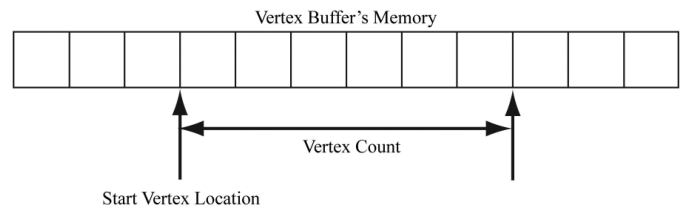
\includegraphics[width=\textwidth]{6-2}
    \centering
    \caption{StartVertexLocation 表示开始绘制的顶点缓冲区的第一个元素。VertexCountPerInstance 表示绘制顶点的个数。}
    \label{fig:6-2}
\end{figure}

DrawInstanced 方法没有制定顶点的基本类型。它们需要被绘制成点,线列表,还是三角列表?回忆5.5.2节,基本拓扑状态是通过 ID3D12GraphicsCommandList::IASetPrimitiveTopology 方法设置的。例:\\
\begin{lstlisting}
mCommandList->IASetPrimitiveTopology(D3D_PRIMITIVE_TOPOLOGY_TRIANGLELIST);
\end{lstlisting}
\end{flushleft}
\section{索引和索引缓冲区(Indices and Index Buffers)}
\begin{flushleft}
与顶点类似,为了让GPU访问索引数组,需要将索引数组放到GPU缓冲区资源中(ID3D12Resource)。我们将存储索引的缓冲区叫索引缓冲区(index buffer)。因为 d3dUtil::CreateDefaultBuffer 方法能通过 void* 作用于一般数据,我们同样使用该方法来创建索引缓冲区(或任何默认缓冲区)。\\
为了将索引缓冲区绑定到管道,我们需要为索引缓冲区资源创建一个索引缓冲区视图。 与顶点缓冲区视图一样,我们不需要一个描述符堆用于索引缓冲区视图。 索引缓冲区视图由D3D12\_INDEX\_BUFFER\_VIEW结构表示:\\
\begin{lstlisting}
typedef struct D3D12_INDEX_BUFFER_VIEW
{
    D3D12_GPU_VIRTUAL_ADDRESS bufferLocation;
    UINT SizeInBytes;
    DXGI_FORMAT Format;
} D3D12_INDEX_BUFFER_VIEW;
\end{lstlisting}
1. BufferLocation: 创建视图的顶点缓冲区资源的虚拟地址。 我们可以使用ID3D12Resource :: GetGPUVirtualAddress方法来获取它。\\
2. SizeInBytes:从BufferLocation开始在索引缓冲区中查看的字节数。\\
3. Format:索引的格式必须是16位索引的 DXGI\_FORMAT\_R16\_UINT 或32位索引的 DXGI\_FORMAT\_R32\_UINT。 如果索引值需要额外的32位范围,则应使用16位索引来减少内存和带宽,并仅使用32位索引。\\
~\\
就顶点缓冲区和其他Direct3D资源而言,在我们可以使用它之前,我们需要将它绑定到管道。 使用 ID3D12CommandList::SetIndexBuffer方法将索引缓冲区绑定到输入汇编程序阶段。 以下代码显示了如何创建一个定义多维数据集三角形的索引缓冲区,创建一个视图并将其绑定到管道:\\
\begin{lstlisting}
std::uint16_t indices[] = {
    // front face
    0, 1, 2,
    0, 2, 3,
    
    // back face
    4, 6, 5,
    4, 7, 6,
    
    // left face
    4, 6, 1,
    4, 1, 0,
    
    // right face
    3, 2, 6,
    3, 6, 7,
    
    // top face
    1, 5, 6,
    1, 6, 2,
    
    // bottom face
    4, 0, 3,
    4, 3, 7
};

const UINT ibByteSize = 36 * sizeof(std::uint16_t);

ComPtr<ID3D12Resource> IndexBufferGPU = nullptr;
ComPtr<ID3D12Resource> IndexBufferUploader = nullptr;
IndexBufferGPU = d3dUtil::CreateDefaultBuffer(md3dDevice.Get(), 
                       mCommandList.Get(), indices, ibByteSize, 
                       IndexBufferUploader);

D3D12_INDEX_BUFFER_VIEW ibv;
ibv.BufferLocation = IndexBufferGPU->GetGPUVirtualAddress();
ibv.Format = DXGI_FORMAT_R16_UINT;
ibv.SizeInBytes = ibByteSize;

mCommandList->IASetIndexBuffer(&ibv);
\end{lstlisting}
最后,使用索引时,用 ID3D12GraphicsCommandList::DrawIndexedInstanced 方法,而不是 DrawInstanced:\\
\begin{lstlisting}
void ID3D12GraphicsCommandList::DrawIndexedInstanced(
    UINT IndexCountPerInstance,
    UINT InstanceCount,
    UINT StartIndexLocation,
    INT BaseVertexLocation,
    UINT StartInstanceLocation);
\end{lstlisting}
1. IndexCountPerInstance:要绘制的索引数量(每个实例)。\\
2. InstanceCount:用于称为实例的高级技术; 现在,将其设置为1,因为我们只绘制一个实例。\\
3. StartIndexLocation:索引缓冲区中的一个元素索引,标志着开始读取索引的起始点。\\
4. BaseVertexLocation:在获取顶点之前,要将此整数值添加到此绘图调用使用的索引中。\\
5. StartInstanceLocation:用于称为实例的高级技术, 目前指定为0。\\
~\\
为了说明这些参数,请考虑以下情况。假设我们有三个对象:一个球体,一个盒子和一个圆柱体。首先,每个对象都有自己的顶点缓冲区和自己的索引缓冲区。每个本地索引缓冲区中的索引都与相应的本地顶点缓冲区有关。现在假设我们将球体,盒子和圆柱体的顶点和索引连接成一个全局顶点和索引缓冲区,如图\ref{fig:6-3}所示。 (可能会连接顶点和索引缓冲区,因为在更改顶点和索引缓冲区时会有一些API开销,这很可能不是瓶颈,但是如果有许多小的顶点和索引缓冲区可以很容易地合并,值得这样做是出于性能方面的原因。)在这个串联之后,索引不再是正确的,因为它们存储索引位置相对于它们相应的本地顶点缓冲区而不是全局索引位置;因此需要重新计算索引以正确地将索引指向全局顶点缓冲区。原始盒子索引是在假设盒子的顶点贯穿索引的情况下计算出来的 0, 1, ..., numBoxVertices-1\\
但是合并之后,就成为:\\
\begin{lstlisting}
firstBoxVertexPos,
firstBoxVertexPos+1,
...,
firstBoxVertexPos+numBoxVertices-1
\end{lstlisting}
 
\begin{figure}[h]
    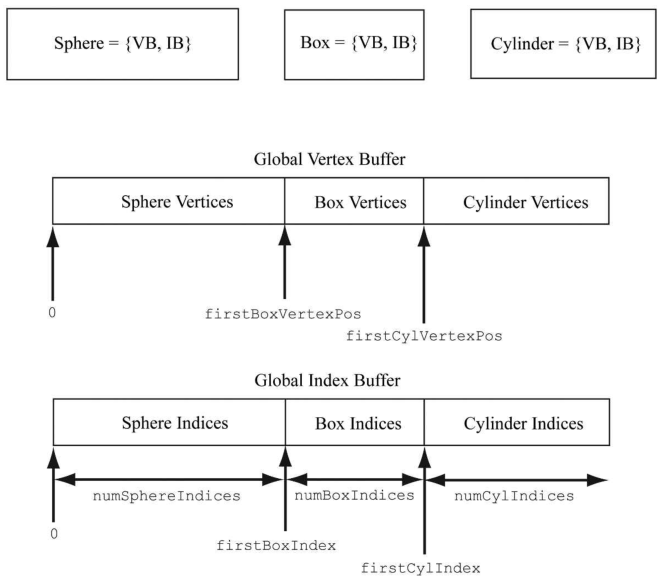
\includegraphics[width=\textwidth]{6-3}
    \centering
    \caption{将几个顶点缓冲区连接成一个大的顶点缓冲区,并将几个索引缓冲区连接成一个大的索引缓冲区。}
    \label{fig:6-3}
\end{figure}

因此,要更新索引,我们需要为每个Box索引添加第一个 firstBoxVertexPos。 同样,我们需要为每个柱面索引添加 firstCylVertexPos。 请注意,球体的指标不需要改变(因为第一个球体顶点位置为零)。 让我们把对象的第一个顶点相对于全局顶点缓冲区的位置称为它的基本顶点位置。 通常,对象的新索引是通过将其基本顶点位置添加到每个索引来计算的。 我们可以让 Direct3D 通过将基本顶点位置传递给 DrawIndexedInstanced 的第四个参数来完成它,而不必自己计算新的索引。\\
然后我们可以用以下三个调用一个接一个地绘制球体,盒子和圆柱体:\\
\begin{lstlisting}
mCmdList->DrawIndexedInstanced(numSphereIndices, 1, 
                               0, 0, 0);
mCmdList->DrawIndexedInstanced(numBoxIndices, 1, 
                               firstBoxIndex, firstBoxVertexPos, 0);
mCmdList->DrawIndexedInstanced(numCylIndices, 1, 
                               firstCylIndex, firstCylVertexPos, 0);
\end{lstlisting}
下一章(chapter)"Shapes"代码样例就使用了这样的技术。
\end{flushleft}

\clearpage
\section{顶点着色器例子(Example Vertex Shader)}
\begin{flushleft}
下面是简单顶点着色器的实现(回忆5.6节):
\end{flushleft}
\begin{lstlisting}
cbuffer cbPerObject : register(b0)
{
    float4x4 gWorldViewProj;
};

void VS(float3 iPosL      : POSITION,
        float4 iColor     : COLOR,
        out float4 oPosH  : SV_POSITION,
        out float4 oColor : COLOR)
{
    // Transform to homogeneous clip space.
    oPosH = mul(float4(iPosL, 1.0f), gWorldViewProj);
    // Just pass vertex color into the pixel shader.
    oColor = iColor;
}
\end{lstlisting}
\begin{flushleft}
着色器使用一种称为高级着色语言(HLSL)的语言编写,它具有与 C++ 类似的语法,因此很容易学习。 附录B提供了对HLSL的简明参考。 我们教授HLSL和编程着色器的方法将以示例为基础。 也就是说,随着本书的进展,我们将介绍我们需要的任何新的HLSL概念,以便实现手头的演示。 着色器通常用基于文本的文件编写,扩展名为.hlsl。\\
顶点着色器是名为VS的函数。 请注意,您可以为顶点着色器指定任何有效的函数名称。 该顶点着色器有四个参数; 前两个是输入参数,后两个是输出参数(由out关键字表示)。 HLSL没有引用或指针,因此要从函数返回多个值,您需要使用结构或输出参数。 在HLSL中,函数始终内联。\\
前两个输入参数构成顶点着色器的输入签名(input signature),并对应于我们用于绘制的自定义顶点结构中的数据成员。 参数语义“:POSITION”和“:COLOR”用于将顶点结构中的元素映射到顶点着色器输入参数,如图\ref{fig:6-4}所示。
\end{flushleft}
\begin{figure}[h]
    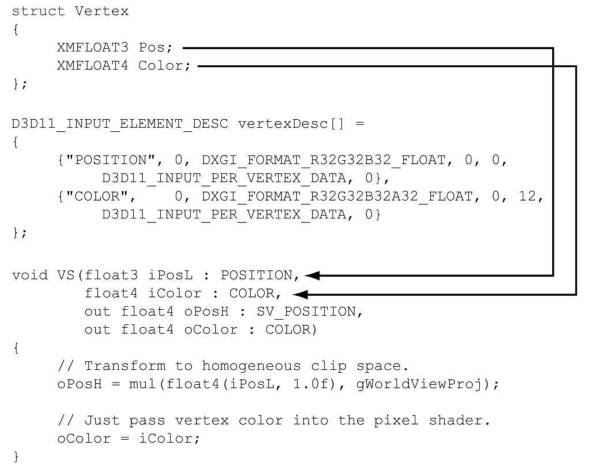
\includegraphics[width=\textwidth]{6-4}
    \centering
    \caption{每个顶点元素都有一个由 D3D12\_INPUT\_ELEMENT\_DESC 数组指定的相关语义。 顶点着色器的每个参数也具有附加的语义。语义用于将顶点元素与顶点着色器参数进行匹配。}
    \label{fig:6-4}
\end{figure}

\begin{flushleft}
输出参数也有附加的语义(“:SV\_POSITION”和“:COLOR”)。 这些用于将顶点着色器输出映射到下一级的相应输入(几何着色器或像素着色器)。 请注意,SV\_POSITION 语义是特殊的(SV代表系统值)。 它用于表示在同构剪辑空间中保存顶点位置的顶点着色器输出元素。 我们必须将SV\_POSITION语义附加到位置输出,因为GPU需要知道这个值,因为它涉及其他属性不涉及的操作,例如剪切,深度测试和光栅化。 非系统值的输出参数的语义名称可以是任何有效的语义名称。\\
第一行通过乘以4x4矩阵 gWorldViewProj 将顶点位置从局部空间转换为齐次剪辑空间:\\
\end{flushleft}
\begin{lstlisting}
// Transform to homogeneous clip space.
oPosH = mul(float4(iPosL, 1.0f), gWorldViewProj);
\end{lstlisting}
\begin{flushleft}
构造函数语法 float4(iPosL,1.0f) 构造一个4D向量,相当于 float4(iPosL.x,iPosL.y,iPosL.z,1.0f); 因为我们知道顶点的位置是点而不是矢量,所以我们在第四个分量中放置 1(w = 1)。float2 和 float3 类型分别代表2D和3D向量。 矩阵变量 gWorldViewProj 存在于所谓的常量缓冲区中,这将在下一节中讨论。 内置函数 mul 用于向量矩阵乘法。顺便提一下,对于不同大小的矩阵乘法,mul 函数是重载(overloaded)的; 例如,您可以使用它来乘以两个4x4矩阵,两个3x3矩阵,或1x3矢量和3x3矩阵。 着色器主体中的最后一行只是将输入颜色复制到输出参数,以便将颜色输入到管道的下一个阶段:\\
\end{flushleft}
\begin{lstlisting}
oColor = iColor;
\end{lstlisting}
\begin{flushleft}
我们可以使用返回类型和输入签名(input signature)的结构(而不是长参数列表)等效地重写上面的顶点着色器:\\
\end{flushleft}
\begin{lstlisting}
cbuffer cbPerObject : register(b0)
{
    float4x4 gWorldViewProj;
};
struct VertexIn
{
    float3 PosL : POSITION;
    float4 Color : COLOR;
};
struct VertexOut
{
    float4 PosH : SV_POSITION;
    float4 Color : COLOR;
};
VertexOut VS(VertexIn vin)
{
    VertexOut vout;
    // Transform to homogeneous clip space.
    vout.PosH = mul(float4(vin.PosL, 1.0f), gWorldViewProj);
    // Just pass vertex color into the pixel shader.
    vout.Color = vin.Color;
    return vout;
}
\end{lstlisting}
\begin{flushleft}
NOTICE: 如果没有几何着色器(第12章中介绍几何着色器),则顶点着色器必须使用 SV\_POSITION 语义输出齐次剪辑空间中的顶点位置,因为这是硬件在离开顶点时期望顶点所在的空间 着色器(如果没有几何着色器)。 如果存在几何着色器,则输出齐次剪辑空间位置的作业可以推迟到几何着色器。\\
~\\
NOTICE: 顶点着色器(或几何着色器)不执行透视分割; 它只是投影矩阵部分。 透视分割将稍后由硬件完成。
\end{flushleft}

\subsection{输入布局描述和输入签名链接(Input Layout Description and Input Signature Linking)}
\begin{flushleft}
从图\ref{fig:6-4}中可以看出,提供给管道的顶点属性之间存在链接,这是由输入布局描述定义的。 如果您输入的顶点不提供顶点着色器所需的所有输入,则会产生错误。 例如,以下顶点着色器输入签名和顶点数据不兼容:\\
\end{flushleft}
\begin{lstlisting}
//––––—
// C++ app code
//––––—
struct Vertex
{
    XMFLOAT3 Pos;
    XMFLOAT4 Color;
};
D3D12_INPUT_ELEMENT_DESC desc[] =
{
    {"POSITION", 0, DXGI_FORMAT_R32G32B32_FLOAT, 0, 0,
                 D3D12_INPUT_PER_VERTEX_DATA, 0},
    {"COLOR",    0, DXGI_FORMAT_R32G32B32A32_FLOAT, 0, 12,
                 D3D12_INPUT_PER_VERTEX_DATA, 0}
};
//––––—
// Vertex shader
//––––—
struct VertexIn
{
    float3 PosL   : POSITION;
    float4 Color  : COLOR;
    float3 Normal : NORMAL;
};
struct VertexOut
{
    float4 PosH  : SV_POSITION;
    float4 Color : COLOR;
};
VertexOut VS(VertexIn vin) {...}
\end{lstlisting}

\begin{flushleft}
正如我们将在6.9节中看到的那样,当我们创建一个 ID3D12PipelineState 对象时,我们必须同时指定输入布局描述和顶点着色器。 然后,Direct3D将验证输入布局描述和顶点着色器是否兼容。\\
顶点数据和输入签名不需要完全匹配。 所需要的是顶点数据提供顶点着色器期望的所有数据。 因此,允许顶点数据提供顶点着色器不使用的附加数据。 也就是说,以下是兼容的:
\end{flushleft}

\begin{lstlisting}
//––––—
// C++ app code
//––––—
struct Vertex
{
   XMFLOAT3 Pos;
   XMFLOAT4 Color;
   XMFLOAT3 Normal;
};
D3D12_INPUT_ELEMENT_DESC desc[] =
{
    {"POSITION", 0, DXGI_FORMAT_R32G32B32_FLOAT, 0, 0,
                 D3D12_INPUT_PER_VERTEX_DATA, 0},
    {"COLOR",    0, DXGI_FORMAT_R32G32B32A32_FLOAT, 0, 12,
                 D3D12_INPUT_PER_VERTEX_DATA, 0},
    {"NORMAL",   0, DXGI_FORMAT_R32G32B32_FLOAT, 0, 28,
                 D3D12_INPUT_PER_VERTEX_DATA, 0 }
};
//––––—
// Vertex shader
//––––—
struct VertexIn
{
    float3 PosL  : POSITION;
    float4 Color : COLOR;
};
struct VertexOut
{
    float4 PosH  : SV_POSITION;
    float4 Color : COLOR;
};
VertexOut VS(VertexIn vin) {...}
\end{lstlisting}
\begin{flushleft}
现在考虑顶点结构和输入签名具有匹配的顶点元素的情况,但颜色属性的类型是不同的:\\
\end{flushleft}
\begin{lstlisting}
//––––—
// C++ app code
//––––—
struct Vertex
{
    XMFLOAT3 Pos;
    XMFLOAT4 Color;
};
D3D12_INPUT_ELEMENT_DESC desc[] =
{
    {"POSITION", 0, DXGI_FORMAT_R32G32B32_FLOAT, 0, 0,
                 D3D12_INPUT_PER_VERTEX_DATA, 0},
    {"COLOR",    0, DXGI_FORMAT_R32G32B32A32_FLOAT, 0, 12,
                 D3D12_INPUT_PER_VERTEX_DATA, 0}
};
//––––—
// Vertex shader
//––––—
struct VertexIn
{
    float3 PosL : POSITION;
    int4 Color  : COLOR;
};
struct VertexOut
{
    float4 PosH  : SV_POSITION;
    float4 Color : COLOR;
};
VertexOut VS(VertexIn vin) {...}
\end{lstlisting}

\begin{flushleft}
这实际上是合法的,因为Direct3D允许重新解释输入寄存器中的位。 但是,VC++调试输出窗口提供以下警告:\\
\end{flushleft}
\begin{lstlisting}
D3D12 WARNING: ID3D11Device::CreateInputLayout: The
provided input signature expects to read an element with
SemanticName/Index: ‘COLOR’/0 and component(s) of the
type ‘int32’. However, the matching entry in the Input
Layout declaration, element[1], specifies mismatched
format: ‘R32G32B32A32_FLOAT’. This is not an error, since
behavior is well defined: The element format determines
what data conversion algorithm gets applied before it
shows up in a shader register. Independently, the shader
input signature defines how the shader will interpret the
data that has been placed in its input registers, with no
change in the bits stored. It is valid for the
application to reinterpret data as a different type once
it is in the vertex shader, so this warning is issued
just in case reinterpretation was not intended by the
author.
\end{lstlisting}

\begin{figure}[h]
	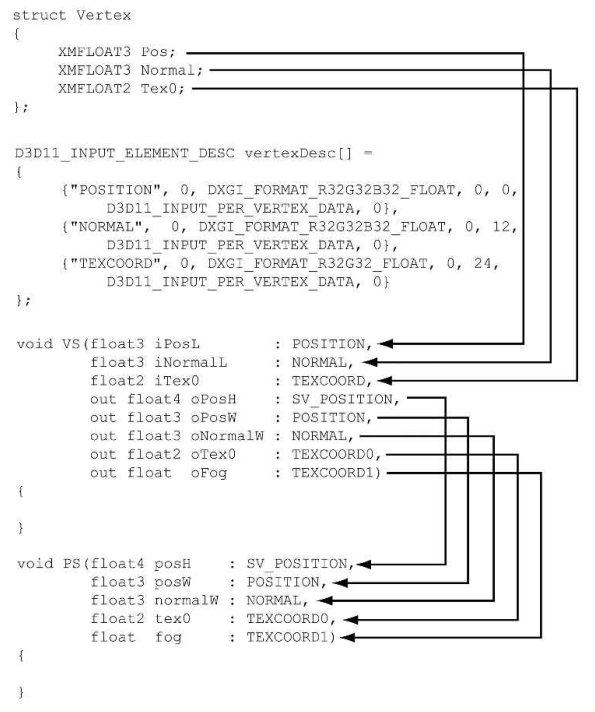
\includegraphics[width=\textwidth]{6-5}
	\centering
	\caption{每个顶点元素都有一个由 D3D12\_INPUT\_ELEMENT\_DESC 数组指定的相关语义。 顶点着色器的每个参数也具有附加的语义。 语义用于将顶点元素与顶点着色器参数进行匹配。 同样,顶点着色器的每个输出都有一个附加的语义,每个像素着色器输入参数都有一个附加的语义。 这些语义用于将顶点着色器输出映射到像素着色器输入参数。}
	\label{fig:6-5}
\end{figure}

\section{像素着色器例子(Example Pixel Shader)}
\begin{flushleft}
如5.10.3节中所述,在光栅化期间,从顶点着色器(或几何着色器)输出的顶点属性在三角形的像素上进行插值。 然后将插值作为输入(5.11节)输入像素着色器。 假设没有几何着色器,图\ref{fig:6-5}说明了到目前为止顶点数据的路径。
\end{flushleft}

\begin{flushleft}
像素着色器就像顶点着色器,因为它是为每个像素片段执行的函数。 给定像素着色器输入,像素着色器的作用是计算像素片段的颜色值。 我们注意到像素片段可能无法存活并使其进入后缓冲区; 例如,它可能被剪裁在像素着色器中(HLSL包含clip 函数,可以丢弃进一步处理的像素片段),被另一个具有较小深度值的像素片段遮挡,或者像素片段可能被稍后丢弃 管道测试就像模板缓冲测试一样。 因此,后缓冲器上的像素可以具有多个像素片段候选; 这是“像素片段”和“像素”的含义之间的区别,尽管有时这些术语可以互换使用,但上下文通常会明确其含义。\\
~\\
NOTICE: 作为硬件优化,在将像素片段设置到像素着色器之前(例如,early-z rejection),可能会使管道拒绝像素片段。 这是首先进行深度测试的地方,并且如果确定像素片段被深度测试遮挡,则跳过像素着色器。 但是,有些情况可能会禁用early-z rejection优化。 例如,如果像素着色器修改像素的深度,则必须执行像素着色器,因为如果像素着色器更改像素着色器,我们实际上不知道像素着色器的深度。\\
~\\
下面是一个简单的像素着色器,它对应于§6.4中给出的顶点着色器。 为完整起见,再次显示顶点着色器。\\
\end{flushleft}
\begin{lstlisting}
cbuffer cbPerObject : register(b0)
{
    float4x4 gWorldViewProj;
};
void VS(float3 iPos : POSITION, 
        float4 iColor : COLOR,
        out float4 oPosH : SV_POSITION,
        out float4 oColor : COLOR)
{
    // Transform to homogeneous clip space.
    oPosH = mul(float4(iPos, 1.0f), gWorldViewProj);
    // Just pass vertex color into the pixel shader.
    oColor = iColor;
}

float4 PS(float4 posH  : SV_POSITION, 
          float4 color : COLOR) : SV_Target
{
    return pin.Color;
}
\end{lstlisting}
\begin{flushleft}
在此示例中,像素着色器仅返回插值颜色值。 请注意,像素着色器输入与顶点着色器输出完全匹配; 这是一项要求。 像素着色器返回4D颜色值,函数参数列表后面的SV\_TARGET语义指示返回值类型应与渲染目标格式匹配。\\
我们可以使用输入/输出结构等效地重写上面的顶点和像素着色器。 符号的不同之处在于我们将语义附加到输入/输出结构的成员,并且我们使用return语句来输出而不是输出参数。
\end{flushleft}
\begin{lstlisting}
cbuffer cbPerObject : register(b0)
{
    float4x4 gWorldViewProj;
};
struct VertexIn
{
    float3 Pos   : POSITION;
    float4 Color : COLOR;
};
struct VertexOut
{
    float4 PosH : SV_POSITION;
    float4 Color : COLOR;
};
VertexOut VS(VertexIn vin)
{
    VertexOut vout;
    // Transform to homogeneous clip space.
    vout.PosH = mul(float4(vin.Pos, 1.0f), gWorldViewProj);
    // Just pass vertex color into the pixel shader.
    vout.Color = vin.Color;
    return vout;
}
float4 PS(VertexOut pin) : SV_Target
{
    return pin.Color;
}
\end{lstlisting}

\section{常量缓冲区(Constant Buffers)}
\subsection{创建常量缓冲区(Creating Constant Buffers)}
\begin{flushleft}
常量缓冲区是GPU资源(ID3D12Resource)的一个例子,其数据内容可在着色器程序中引用。 正如我们将在本书中学习的那样,着色器程序中也可以引用纹理和其他类型的缓冲区资源。 6.4节中的示例顶点着色器的代码如下:
\begin{lstlisting}
cbuffer cbPerObject: register(b0)
{
    float4x4 gWorldViewProj;
}
\end{lstlisting}
此代码引用一个名为cbPerObject的cbuffer对象(常量缓冲区)。 在这个例子中,常量缓冲区存储一个名为gWorldViewProj的4x4矩阵,表示用于将点从本地空间转换为同类剪辑空间的组合世界,视图和投影矩阵。 在HLSL中,4x4矩阵由内置的float4x4类型声明; 要声明3x4矩阵和2x4矩阵,例如,您将分别使用float3x4和float2x2类型。\\
与顶点和索引缓冲区不同,常量缓冲区通常由CPU每帧更新一次。 例如,如果摄像机每帧移动一次,则每帧必须使用新的视图矩阵更新常量缓冲区。 因此,我们在上传堆而不是默认堆中创建常量缓冲区,以便我们可以从CPU更新内容。\\
常量缓冲区也有特殊的硬件要求,它们的大小必须是最小硬件分配大小(256字节)的倍数。\\
通常我们需要多个相同类型的常量缓冲区。 例如,上面的常量缓冲区cbPerObject存储每个对象不同的常量,所以如果我们有n个对象,那么我们将需要n个这种类型的常量缓冲区。 以下代码显示了我们如何创建一个存储NumElements多个常量缓冲区的缓冲区:
\begin{lstlisting}
struct ObjectConstants
{
    DirectX::XMFLOAT4X4 WorldViewProj = MathHelper::Identity4x4();
};

UINT elementByteSize = d3dUtil::CalcConstantBufferByteSize(
                                     sizeof(ObjectConstants));

ComPtr<ID3D12Resource> mUploadCBuffer;
device->CreateCommittedResource(
    &CB3DX12_HEAP_PROPERTIES(D3D12_HEAP_TYPE_UPLOAD), 
    D3D12_HEAP_FLAG_NONE, 
    &CD3DX12_RESOURCE_DESC::Buffer(elementByteSize * NumElements),
    D3D12_RESOURCE_STATE_GENERIC_READ,
    nullptr, 
    IID_PPV_ARGS(&mUploadCBuffer));
\end{lstlisting}
我们可以将mUploadCBuffer视为存储ObjectConstants类型的常量缓冲区数组(使用填充为256的倍数)。 当需要绘制一个对象时,我们只需将一个常量缓冲区视图(CBV)绑定到缓冲区的一个存储该对象常量的子区域。 请注意,我们经常会调用缓冲区mUploadCBuffer作为常量缓冲区,因为它存储了一个常量缓冲区数组。\\
工具函数 d3dUtil::CalcConstantBufferByteSize 会进行算术运算将缓冲区的字节大小舍入为最小硬件分配大小(256字节)的倍数:\\
\begin{lstlisting}
static UINT CalcConstantBufferByteSize(UINT byteSize)
{
    // Constant buffers must be a multiple of the minimum hardware
    // allocation size (usually 256 bytes).  So round up to nearest
    // multiple of 256.  We do this by adding 255 and then masking off
    // the lower 2 bytes which store all bits < 256.
    // Example: Suppose byteSize = 300.
    // (300 + 255) & ~255
    // 555 & ~255
    // 0x022B & ~0x00ff
    // 0x022B & 0xff00
    // 0x0200
    // 512
    return (byteSize + 255) & ~255;
}
\end{lstlisting}
NOTICE: 即使我们以256的倍数分配常量数据,也不需要在HLSL结构中明确填充相应的常量数据,因为它是隐式完成的:\\
\begin{lstlisting}
// Implicitly padded to 256 bytes.
cbuffer cbPerObject : register(b0)
{
    float4x4 gWorldViewProj;
};

// Explicitly padded to 256 bytes.
cbuffer cbPerObject : register(b0)
{
    float4x4 gWorldViewProj;
    float4x4 Pad0;
    float4x4 Pad1;
    float4x4 Pad1;
}
\end{lstlisting}
NOTICE: 为避免处理将常量缓冲区元素舍入为256字节的倍数,可以明确地将所有常量缓冲区结构填充为256字节的整数倍。\\
~\\
Direct3D 12推出了着色器模型5.1。 Shader model 5.1引入了一种替代HLSL语法来定义一个常量缓冲区,如下所示:\\
\begin{lstlisting}
struct ObjectConstants
{
    float4x4 gWorldViewProj;
    uint matIndex;
};
ConstantBuffer<ObjectConstants> gObjConstants : register(b0);
\end{lstlisting}
这里常量缓冲区的数据元素只是在一个单独的结构中定义,然后从该结构创建一个常量缓冲区。 然后使用数据成员语法在着色器中访问常量缓冲区的字段:\\
\begin{lstlisting}
uint index = gObjConstants.matIndex;
\end{lstlisting}
\end{flushleft}

\subsection{更新常量缓冲区(Updating Constant Buffers)}
\begin{flushleft}
因为一个常量缓冲区是由 D3D12\_HEAP\_TYPE\_UPLOAD 的堆类型创建的,所以我们能从CPU上传常量缓冲区资源。为了做到这一点,要先通过 Map 方法获得资源数据的指针:\\
\begin{lstlisting}
ComPtr<ID3D12Resource> mUploadBuffer;
BYTE* mMappedData = nullptr;
mUploadBuffer->Map(0, nullptr, reinterpret_cast<void**>(&mMappedData));
\end{lstlisting}
第一个参数表示要映射的子资源索引。 对于一个缓冲区,唯一的子资源就是缓冲区本身,所以我们将其设置为0.第二个参数是一个指向D3D12\_RANGE结构的可选指针,该结构描述要映射的内存范围; 指定null映射整个资源。 第三个参数返回一个指向映射数据的指针。 要将数据从系统内存复制到常量缓冲区,我们只需执行一个memcpy即可:\\
\begin{lstlisting}
memcpy(mMappedData, &data, dataSizeInBytes);
\end{lstlisting}
当我们处理完常量缓冲区后,我们应该在释放内存之前 Unmap 它:\\
\begin{lstlisting}
if (mUploadBuffer != nullptr)
    mUploadBuffer->Unmap(0, nullptr);
mMappedData = nullptr;
\end{lstlisting}
Unmap 的第一个参数表示要映射的子资源索引,对于 buffer,这里设为0。第二个参数是一个指向D3D12\_RANGE结构的可选指针,该结构描述要unmap的内存范围; 指定null,unmap 整个资源。
\end{flushleft}

\subsection{上传缓冲区帮助工具(Upload Buffer Helper)}
\begin{flushleft}
在上传缓冲区周围构建一个简单的包装器很方便。 我们在UploadBuffer.h中定义了以下类,以便更轻松地处理上传缓冲区。 它为我们处理上传缓冲区资源的构建和销毁,处理映射和取消映射资源,并提供CopyData方法来更新缓冲区中的特定元素。 当我们需要从CPU更改上传缓冲区的内容时(例如,当视图矩阵发生变化时),我们使用CopyData方法。 请注意,这个类可以用于任何上传缓冲区,不一定是一个常量缓冲区。 但是,如果我们将它用于常量缓冲区,则需要通过isConstantBuffer构造函数参数进行指示。 如果它正在存储一个常量缓冲区,那么它会自动填充内存,使每个常量缓冲区为256字节的倍数。
\end{flushleft}
\begin{lstlisting}
template<typename T>
class UploadBuffer
{
public:
    UploadBuffer(ID3D12Device* device, UINT elementCount, 
                 bool isConstantBuffer) 
                 : mIsConstantBuffer(isConstantBuffer)
    {
        mElementByteSize = sizeof(T);

        // Constant buffer elements need to be multiples of 256 bytes.
        // This is because the hardware can only view constant data 
        // at m*256 byte offsets and of n*256 byte lengths. 
        // typedef struct D3D12_CONSTANT_BUFFER_VIEW_DESC {
        // UINT64 OffsetInBytes; // multiple of 256
        // UINT   SizeInBytes;   // multiple of 256
        // } D3D12_CONSTANT_BUFFER_VIEW_DESC;
        if(isConstantBuffer)
            mElementByteSize = d3dUtil::CalcConstantBufferByteSize(
                                                         sizeof(T));

        ThrowIfFailed(device->CreateCommittedResource(
            &CD3DX12_HEAP_PROPERTIES(D3D12_HEAP_TYPE_UPLOAD),
            D3D12_HEAP_FLAG_NONE,
            &CD3DX12_RESOURCE_DESC::Buffer(mElementByteSize*elementCount),
            D3D12_RESOURCE_STATE_GENERIC_READ,
            nullptr,
            IID_PPV_ARGS(&mUploadBuffer)));

        ThrowIfFailed(mUploadBuffer->Map(0, nullptr, 
                          reinterpret_cast<void**>(&mMappedData)));

        // We do not need to unmap until we are done with the resource.
        // However, we must not write to
        // the resource while it is in use by the GPU 
        // (so we must use synchronization techniques).
    }

    UploadBuffer(const UploadBuffer& rhs) = delete;
    UploadBuffer& operator=(const UploadBuffer& rhs) = delete;
    ~UploadBuffer()
    {
        if(mUploadBuffer != nullptr)
            mUploadBuffer->Unmap(0, nullptr);

        mMappedData = nullptr;
    }

    ID3D12Resource* Resource()const
    {
        return mUploadBuffer.Get();
    }

    void CopyData(int elementIndex, const T& data)
    {
        memcpy(&mMappedData[elementIndex*mElementByteSize], &data, 
                                                         sizeof(T));
    }

private:
    Microsoft::WRL::ComPtr<ID3D12Resource> mUploadBuffer;
    BYTE* mMappedData = nullptr;

    UINT mElementByteSize = 0;
    bool mIsConstantBuffer = false;
};
\end{lstlisting}
\begin{flushleft}
通常情况下,对象的世界矩阵在移动/旋转/缩放时会发生变化,视图矩阵会在摄像机移动/旋转时发生变化,并且在窗口大小调整时投影矩阵发生变化。 在本章的演示中,我们允许用户使用鼠标旋转和移动摄像头,并且我们在更新函数的每一帧中使用新的视图矩阵更新组合的世界视图投影矩阵:
\end{flushleft}
\begin{lstlisting}
void BoxApp::OnMouseMove(WPARAM btnState, int x, int y)
TODO....
\end{lstlisting}

\subsection{常量缓冲区描述符(Constant Buffer Descriptor)}
\begin{flushleft}
回想一下4.1.6节,我们通过描述符对象将资源绑定到渲染管道。 到目前为止,我们已经使用渲染目标,深度/模板缓冲区,顶点和索引缓冲区的描述符/视图。 我们还需要描述符来将常量缓冲区绑定到管道。 常量缓冲区描述符位于D3D12\_DESCRIPTOR\_HEAP\_TYPE\_CBV\_SRV\_UAV类型的描述符堆中。 这样的堆可以存储常量缓冲区,着色器资源和无序访问描述符的混合。 为了存储这些新类型的描述符,我们需要创建一个新的描述符堆类型:\\
\end{flushleft}
\begin{lstlisting}
D3D12_DESCRIPTOR_HEAP_DESC cbvHeapDesc;
cbvHeapDesc.NumDescriptors = 1;
cbvHeapDesc.Type = D3D12_DESCRIPTOR_HEAP_TYPE_CBV_SRV_UAV;
cbvHeapDesc.Flags = D3D12_DESCRIPTOR_HEAP_FLAG_SHADER_VISIBLE;
cbvHeapDesc.NodeMask = 0;

ComPtr<ID3D12DescriptorHeap> mCbvHeap;
md3dDevice->CreateDescriptorHeap(&cbvHeapDesc, IID_PPV_ARGS(&mCbvHeap));
\end{lstlisting}
\begin{flushleft}
这段代码与我们如何创建渲染目标和深度/模板缓冲区描述符堆相似。 然而,一个重要的区别是我们指定了D3D12\_DESCRIPTOR\_HEAP\_FLAG\_SHADER\_VISIBLE标志来表示这些描述符将被着色器程序访问。 在4.1.6节的演示中,我们没有SRV或UAV描述符,我们只绘制一个对象; 因此,我们只需要1个描述符来存储1个CBV。\\
通过填写一个D3D12\_CONSTANT\_BUFFER\_VIEW\_DESC实例并调用ID3D12Device::CreateConstantBufferView来创建一个常量缓冲区视图:\\
\end{flushleft}
\begin{lstlisting}
// Constant data per-object.
struct ObjectConstants
{
    XMFLOAT4X4 WorldViewProj = MathHelper::Identity4x4();
};

// Constant buffer to store the constants of n object.
std::unique_ptr<UploadBuffer<ObjectConstants>> mObjectCB = nullptr;
mObjectCB = std::make_unique<UploadBuffer<ObjectConstants>>(
                                        md3dDevice.Get(), n, true);

UINT objCBByteSize = d3dUtil::CalcConstantBufferByteSize(
                                           sizeof(ObjectConstants));

// Address to start of the buffer (0th constant buffer).
D3D12_CPU_VIRTUAL_ADDRESS cbAddress = mObjectCB->Resource()
                                          ->GetGPUVirtualAddress();

// Offset to the ith object constant buffer in the buffer.
int boxCBufIndex = i;
cbAddress += boxCBufIndex * objCBByteSize;

D3D12_CONSTANT_BUFFER_VIEW_DESC cbvDesc;
cbvDesc.BufferLocation = cbAddress;
cbvDesc.SizeInBytes = d3dUtil::CalcConstantBufferByteSize(
                                           sizeof(ObjectConstants));

md3dDevice->CreateConstantBufferView(&cbvDesc, mCbvHeap
                             ->GetCPUDescriptorHandleForHeapStart());
\end{lstlisting}
\begin{flushleft}
D3D12\_CONSTANT\_BUFFER\_VIEW\_DESC 结构描述了要绑定到HLSL常量缓冲区结构的常量缓冲区资源的子集。 如前所述,通常一个常量缓冲区存储n个对象的每个对象常量数组,但我们可以通过使用 BufferLocation 和 SizeInBytes 来获取第i个对象常量数据的视图。 由于硬件要求,D3D12\_CONSTANT\_BUFFER\_VIEW\_DESC::SizeInBytes 和D3D12\_CONSTANT\_BUFFER\_VIEW\_DESC::OffsetInBytes 成员必须为256个字节的倍数。 例如,如果您指定了64,那么您将得到以下调试错误:\\
\end{flushleft}
\begin{lstlisting}
D3D12 ERROR: ID3D12Device::CreateConstantBufferView: 
             SizeInBytes of 64 is invalid. 
             Device requires SizeInBytes be multiple of 256.

D3D12 ERROR: ID3D12Device::CreateConstantBufferView: 
             OffsetInBytes of 64 is invalid. 
             Device requires OffsetInBytes be a multiple of 256.
\end{lstlisting}

\subsection{根签名和描述符表(Root Signature and Descriptor Tables)}
\begin{flushleft}
通常,不同的着色器程序会希望在执行绘制调用之前将不同的资源绑定到渲染管道。 资源被绑定到特定的寄存器插槽,在那里它们可以被着色器程序访问。 例如,以前的顶点和像素着色器只需要一个常量缓冲区被绑定到寄存器b0。 本书稍后将使用的更高级的顶点和像素着色器集合将期望将几个常量缓冲区,纹理和采样器绑定到各种寄存器槽:\\
\begin{lstlisting}
// Texture resourcce bound to texture register slot 0.
Texture2D gDiffuseMap : register(t0);

// Sampler resources bound to sampler register slots 0-5.
SamplerState gsamPointWrap        : register(s0);
SamplerState gsamPointClamp       : register(s1);
SamplerState gsamLinearWrap       : register(s2);
SamplerState gsamLinearClamp      : register(s3);
SamplerState gsamAnisotropicWrap  : register(s4);
SamplerState gsamAnisotropicClamp : register(s5);

// cbuffer resource bound to cbuffer register slots 0-2
cbuffer cbPerObject : register(b0)
{
    float4x4 gWorld;
    float4x4 gTexTransform;
};

// Constant data that varies per material.
cbuffer cbPass : register(b1)
{
    float4x4 gView;
    float4x4 gProj;
    [...] // Other fields omitted for brevity.
};

cbuffer cbMaterial : register(b2)
{
    float4   gDiffuseAlbedo;
    float3   gFresnelR0;
    float    gRoughness;
    float4x4 gMatTransform;
};
\end{lstlisting}
根签名定义了在绘制调用可以执行之前应用程序将绑定到渲染管道的资源以及这些资源被映射到着色器输入寄存器的位置。 根签名必须与将要使用的着色器兼容(即,根签名必须提供着色器期望在绘制调用执行之前绑定到渲染管道的所有资源); 这将在创建管道状态对象时进行验证(6.9节)。 不同的绘制调用可能会使用一组不同的着色器程序,这需要不同的根签名。\\
~\\
NOTICE: 如果我们将着色器程序看作函数,并将着色器期望的输入资源作为函数参数来考虑,那么根签名可以被认为是定义函数签名(因此称为根签名)。 通过绑定不同的资源作为参数,着色器输出将会不同。 所以,例如,顶点着色器将取决于输入到着色器的实际顶点以及绑定资源。\\
~\\
Direct3D中的根签名由ID3D12RootSignature接口表示。 它由一组根参数定义,这些参数描述了着色器对绘制调用所期望的资源。 根参数可以是根常量,根描述符或描述符表。 我们将在下一章讨论根常量和根描述符; 在本章中,我们将只使用描述符表。 描述符表指定描述符堆中描述符的连续范围。\\
下面的代码创建一个根签名,该签名具有一个根描述符表,该描述符表足够大以存储一个CBV(常量缓冲区视图):\\
\begin{lstlisting}
// Root parameter can be a table, root descriptor or root constants.
CD3DX12_ROOT_PARAMETER slotRootParameter[1];

// Create a single descriptor table of CBVs.
CD3DX12_DESCRIPTOR_RANGE cbvTable;
cbvTable.Init(
    D3D12_DESCRIPTOR_RANGE_TYPE_CBV,
    1,  // Number of descriptors in table
    0); // base shader register arguments are bound to 
        // for this root parameter

slotRootParameter[0].InitAsDescriptorTable(
    1,          // Number of ranges
    &cbvTable); // Pointer to array of ranges

// A root signature is an array of root parameters.
CD3DX12_ROOT_SIGNATURE_DESC rootSigDesc(1, 
    slotRootParameter, 0, nullptr, 
    D3D12_ROOT_SIGNATURE_FLAG_ALLOW_INPUT_ASSEMBLER_INPUT);

// create a root signature with a single slot with pints to a
// descriptor range consisting of a single constant buffer.
ComPtr<ID3DBlob> serializedRootSig = nullptr;
ComPtr<ID3DBlob> errorBlob = nullptr;

HRESULT hr = D3D12SerializeRootSignature(&rootSigDesc, 
    D3D_ROOT_SIGNATURE_VERSION_1,
    serializedRootSig.GetAddressOf(),
    errorBlob.GetAddressOf());

ThrowIfFailed(md3dDevice->CreateRootSignature(
    0,
    serializedRootSig->GetBufferPointer(),
    serializedRootSig->GetBufferSize(),
    IID_PPV_ARGS(&mRootSignature)));
\end{lstlisting}
下一章我们再解释 CD3DX12\_ROOT\_PARAMETER 和 CD3DX12\_DESCRIPTOR\_RANGE,现在仅理解如下代码:\\
\begin{lstlisting}
CD3DX12_ROOT_PARAMETER slotRootParameter[1];

CD3DX12_DESCRIPTOR_RANGE cbvTable;
cbvTable.Init(
    D3D12_DESCRIPTOR_RANGE_TYPE_CBV, // table type
    1,  // Number of descriptors in table
    0); // base shader register arguments are bound to 
        // for this root parameter

slotRootParameter[0].InitAsDescriptorTable(
    1,          // Number of ranges
    &cbvTable); // Pointer to array of ranges
\end{lstlisting}
创建一个根参数,该参数需要1个CBV的描述符表被绑定到常量缓冲寄存器0(即,HLSL代码中的寄存器(b0))。\\
~\\
NOTICE: 我们在本章中的根签名示例非常简单。 在本书中,我们将看到许多根签名的例子,并且它们会根据需要增加复杂性。
~\\
根签名仅定义应用程序将绑定到渲染管道的资源; 它实际上并没有做任何资源绑定。 一旦使用命令列表设置了根签名,我们使用ID3D12GraphicsCommandList::SetGraphicsRootDescriptorTable将描述符表绑定到管道:\\
\begin{lstlisting}
void ID3D12GraphicsCommandList::SetGraphicsRootDescriptorTable(
    UINT RootParameterIndex,
    D3D12_GPU_DESCRIPTOR_HANDLE BaseDescriptor);
\end{lstlisting}
1. RootParameterIndex: 设置根参数的索引。\\
2. BaseDescriptor: 处理堆中的描述符,指定要设置的表中的第一个描述符。 例如,如果根签名指定该表具有五个描述符,则将BaseDescriptor和堆中接下来的四个描述符设置为此根表。\\
以下代码将根签名和CBV堆设置为命令列表,并将描述符表设置为标识要绑定到管道的资源:\\
\begin{lstlisting}
mCommandList->SetGraphicsRootSignature(mRootSignature.Get());
ID3D12DescriptorHeap* descriptorHeaps[] = {mCbvHeap.Get()};
mCommandList->SetDescriptorHeaps(_countof(descriptorHeaps), descriptorHeaps);

// Offset the CBV we want to use for this draw call.
CD3DX12_GPU_DESCRIPTOR_HANDLE cbv(mCbvHeap->GetGPUDescriptorHandleForheapStart());
cbv.Offset(cbvIndex, mCbvSrvUavDescriptorSize);
mCommandList->SetGraphicsRootDescriptorTable(0, cbv);
\end{lstlisting}
~\\
NOTICE: 为了提高性能,请尽可能缩小根签名,并尽量减少每个渲染帧更改根签名的次数。\\
NOTICE: 只要内容的任何部分在绘图/分派调用之间发生变化,应用程序绑定的根签名(描述符表,根常量和根描述符)的内容就会自动得到D3D12驱动程序的版本控制。 所以每个绘图/分派都会得到一个独特的全套根签名状态。\\
NOTICE: 如果更改根签名,则会丢失所有现有的绑定。 也就是说,您需要重新绑定新根签名所需的所有资源。
\end{flushleft}

\section{编译着色器(Compiling Shaders)}
\begin{flushleft}
在Direct3D中,着色器程序必须首先编译为便携式字节码。 然后,图形驱动程序将获取该字节码并将其重新编译为系统GPU [ATI1]的最佳本机指令。 在运行时,我们可以使用以下函数编译着色器:\\
\begin{lstlisting}
HRESULT D3DCompileFromFile(
    LPCWSTR pFileName,
    const D3D_SHADER_MACRO *pDefines,
    ID3DInclude *pInclude,
    LPCSTR pEntrypoint,
    LPCSTR pTarget,
    UINT Flags1,
    UINT Flags2,
    ID3DBlob **ppCode,
    ID3DBlob **ppErrorMsgs);
\end{lstlisting}
1. pFileName: .hlsl 后缀的文件名称,该文件包含了需要编译的HLSL源代码。\\
2. pDefines: 不使用的高级选项; 请参阅SDK文档。 我们在本书中总是指定null。\\
3. pInclude: 不使用的高级选项; 请参阅SDK文档。 我们在本书中总是指定null。\\
4. pEntrypoint: 着色器入口点的函数名称。 一个.hlsl可以包含多个着色器程序(例如,一个顶点着色器和一个像素着色器),所以我们需要指定我们想要编译的特定着色器的入口点。\\
5. pTarget: 指定我们正在使用的着色器程序类型和版本的字符串。在本书中,我们的目标是版本5.0和5.1。\\
\begin{itemize}
  \item a) vs\_5\_0 和 vs\_5\_1: 顶点着色器(vertex shader) 5.0 和 5.1。
  \item b) hs\_5\_0 和 hs\_5\_1: 外壳着色器(hull shader) 5.0 和 5.1。
  \item c) ds\_5\_0 和 ds\_5\_1: 域着色器(domain shader) 5.0 和 5.1。
  \item c) gs\_5\_0 和 gs\_5\_1: 几何着色器(geometry shader) 5.0 和 5.1。
  \item c) ps\_5\_0 和 ps\_5\_1: 像素着色器(pixel shader) 5.0 和 5.1。
  \item c) cs\_5\_0 和 cs\_5\_1: 计算着色器(compute shader) 5.0 和 5.1。
\end{itemize}
5. Flags1: 用于指定应该如何编译着色器代码的标志。 SDK文档中列出了相当多的这些标志,但本书中仅有的两个标志是:\\
\begin{itemize}
  \item a) D3DCOMPILE\_DEBUG: 以DEBUG模式编译着色器。
  \item b) D3DCOMPILE\_SKIP\_OPTIMIZATION: 让编译器跳过优化(调试时很有用)。
\end{itemize}
8. ppCode: 返回一个指针,指向存储编译着色器对象字节码的ID3DBlob数据结构。\\
9. ppErrorMsgs: 返回一个指针,只想存储编译错误字符串的ID3DBlob数据结构。\\
ID3DBlob 类型是一个泛化(通用)的内存块(chunck of memory),它有两个方法:\\
\begin{itemize}
    \item 1. LPVOID GetBufferPointer: 返回一个 void* 值,所以它在使用前必须被转换为合适的类型(参见下面的例子)。
    \item 2. SIZE\_T GetBufferSize: 返回缓冲区的字节大小。
\end{itemize}
为了支持错误输出,d3dUtil.h/.cpp 提供了以下函数用来运行期编译着色器:\\
\begin{lstlisting}
ComPtr<ID3DBlob> d3dUtil::CompileShader(
    const std::wstring& filename,
    const D3D_SHADER_MACRO* defines,
    const std::string& entrypoint,
    const std::string& target)
{
    UINT compileFlags = 0;
#if defined(DEBUG) || defined(_DEBUG)  
    compileFlags = D3DCOMPILE_DEBUG | D3DCOMPILE_SKIP_OPTIMIZATION;
#endif

    HRESULT hr = S_OK;

    ComPtr<ID3DBlob> byteCode = nullptr;
    ComPtr<ID3DBlob> errors;
    hr = D3DCompileFromFile(filename.c_str(), defines, 
                            D3D_COMPILE_STANDARD_FILE_INCLUDE,
                            entrypoint.c_str(), target.c_str(), 
                            compileFlags, 0, &byteCode, &errors);

    if(errors != nullptr)
        OutputDebugStringA((char*)errors->GetBufferPointer());

    ThrowIfFailed(hr);

    return byteCode;
}
// Here is an example of calling this function:
ComPtr<ID3DBlob> mvsByteCode = nullptr;
ComPtr<ID3DBlob> mpsByteCode = nullptr;
mvsByteCode = d3dUtil::CompileShader(L"Shaders\color.hlsl", 
                                     nullptr, "VS", "vs_5_0");
mpsByteCode = d3dUtil::CompileShader(L"Shaders\color.hlsl", 
                                     nullptr, "PS", "ps_5_0");
\end{lstlisting}
HLSL错误和警告将通过ppErrorMsgs参数返回。 例如,如果我们拼错了mul函数,那么我们得到以下错误输出到调试窗口:\\
\begin{lstlisting}
Shaders\color.hlsl(29, 14-55): error X3004: undecleared identifier 'mu'
\end{lstlisting}
编译着色器不会将其绑定到渲染管道以供使用。 我们将在6.9节中看到如何做到这一点。
\end{flushleft}

\subsection{离线编译(Offline Compilation)}
\begin{flushleft}
除了在运行期编译着色器,还可以通过离线方式分步骤编译(例如构建步骤或作为资产内容管道过程的一部分)。以下是这么做的原因:\\
\begin{itemize}
    \item 1. 对于复杂的着色器,编译可能需要很长时间。 因此,离线编译将使您的加载时间更快。
    \item 2. 在编译时期提早看到着色器的编译错误比在运行时期方便。
    \item 3. Windows8 APP 商店必须使用离线编译。
\end{itemize}
对编译着色器使用.cso(compiled shader object)扩展名是常见做法。\\
要离线编译着色器,我们使用DirectX附带的FXC工具。 这是一个命令行工具。 要通过入口点分别编译VS和PS(保存在color.hlsl中的顶点和像素着色器),为了debug,我们将编写指令:\\
\begin{lstlisting}
fxc "color.hlsl" /Od /Zi /T vs_5_0 /E "VS" /Fo 
    "color_vs.cso" /Fc "color_vs.asm"
fxc "color.hlsl" /Od /Zi /T ps_5_0 /E "PS" /Fo 
    "color_ps.cso" /Fc "color_ps.asm"
\end{lstlisting}
要通过入口点分别编译VS和PS(保存在color.hlsl中的顶点和像素着色器),为了发布,我们将编写指令:\\
\begin{lstlisting}
fxc "color.hlsl" /T vs_5_0 /E "VS" /Fo "color_vs.cso" /Fc "color_vs.asm"
fxc "color.hlsl" /T ps_5_0 /E "PS" /Fo "color_ps.cso" /Fc "color_ps.asm"
\end{lstlisting}
\begin{tabular}{|p{5em}|p{35em}|} 
\hline
Parameter & Description\\ 
\hline
/Od & Disables optimizations(useful for debugging).\\ 
\hline
/Zi & Enables debug information\\
\hline 
/T<string> & Shader type and target version.\\
\hline 
/E<string> & Shader entry point.\\
\hline 
/Fo<string> & Compiled shader object bytecode.\\
\hline 
/Fc<string> & Outputs an assembly file listing (useful for debugging, checking instruction counts, seeing what kind of code is being generated).\\ 
\hline
\end{tabular}
如果您尝试编译语法错误的着色器,FXC会将错误/警告输出到命令窗口。 例如,如果我们在color.hlsl效果文件中错误地命名了一个变量:\\
\begin{lstlisting}
// Should be gWorldViewProj, not worldViewProj!
vout.PosH = mul(float4(vin.Pos, 1.0f), worldViewProj);
\end{lstlisting}
然后,我们从输出窗口中看到这一个错误的日志(最重要的错误是修复的关键错误):\\
\begin{lstlisting}
color.hlsl(29,42-54): error X3004: undeclared identifier 'worldViewProj'
color.hlsl(29,14-55): error X3013: 'mul': no matching 2 parameter 
                      intrinsic function
color.hlsl(29,14-55): error X3013: Possible intriinsic function are:
color.hlsl(29,14-55): error X3013: mul(float|half...
\end{lstlisting}
在编译期看到错误比运行期方便得多。\\
我们已经展示了如何将顶点和像素着色器离线编译为.cso文件。 因此,我们不再需要在运行时执行它(即,我们不需要调用D3DCompileFromFile)。 但是,我们仍然需要将编译的着色器对象字节码从.cso文件加载到我们的应用程序中。 这可以使用标准C ++文件输入机制完成,如下所示:\\
\begin{lstlisting}
ComPtr<ID3DBlob> d3dUtil::LoadBinary(const std::wstring& filename)
{
    std::ifstream fin(filename, std::ios::binary);
    
    fin.seekg(0, std::ios_base::end);
    std::ifstream::pos_type size = (int)fin.tellg();
    fin.seekg(0, std::ios_base::beg);
    
    ComPtr<ID3DBlob> blob;
    ThrowIfFailed(D3DCreateBlob(size, blob.GetAddressOf()));
    
    fin.read((char*)blob->GetBufferPointer(), size);
    fin.close();

    return blob;
}
...
ComPtr<ID3DBlob> mvsByteCode = d3dUtil::LoadBinary(L"Shaders\color_vs.cso");
ComPtr<ID3DBlob> mpsByteCode = d3dUtil::LoadBinary(L"Shaders\color_ps.cso");
\end{lstlisting}
\end{flushleft}

\subsection{生成汇编代码(Generated Assembly)}
\begin{flushleft}
FXC的/Fc可选参数能生成可移植汇编代码。 随时查看着色器的汇编对于检查着色器指令计数以及查看正在生成的代码类型非常有用 - 有时它可能与你所期望的不同。 例如,如果你的HLSL代码中有条件语句,那么你可能希望汇编代码中存在分支指令。 在早期GPU编程中,着色器中的分支代价过高,因此编译器有时会通过对两个分支进行评估来平滑(flatten)条件语句,然后在两者之间进行插值以选择正确的答案。 也就是说,下面的代码会给出相同的答案:\\
~\\
\begin{tabular}{|p{20em}|p{20em}|} 
\hline
Conditional & Flattened\\ 
\hline
\begin{lstlisting}
float x = 0;

// s == 1 (true) or s == 0 (false)
if (s)
  x = sqrt(y);
else
  x = 2*y;
\end{lstlisting}
&
\begin{lstlisting}
float a = 2*y;
float b = sqrt(y);
float x = a + s * (b - a);
// s == 1: x = a + b - a = b = sqrt(y);
// s == 0: x = a + 0*(b - a) = a = 2*y;
\end{lstlisting}\\
\hline
\end{tabular}
所以Flattened方法给了我们相同的结果,没有任何分支,但是没有看到汇编代码,我们不知道是否发生了扁平化,或者是否生成了真正的分支指令。 问题的关键在于,有时候你想看看程序集来看看到底发生了什么。 以下是在color.hlsl中为顶点着色器生成的汇编示例:\\
\begin{lstlisting}
//
// Generated by Microsoft (R) HLSL Shader Compiler 6.4.9844.0
//
//
// Buffer Definitions:
//
// cbuffer cbPerObject
// {
//     float4x4 gWorldViewProj; // Offset: 0 Size: 64
// }
//
// Resource Bindings:
//
// Name         Type     Format Dim  Slot Elements
// ------------ -------- ------ ---- ---- --------
// cbPerObject  cbuffer  NA     NA   0    1
//
// Input signature:
// Name         Index Mask Register SysValue Format Used
// ------------ ----- ---- -------- -------- ------ -----
// POSITION     0     xyz  0        NONE     float  xyz
// COLOR        0     xyzw 1        NONE     float  xyzw
//
// Output signature:
// Name         Index Mask Register SysValue Format Used
// ------------ ----- ---- -------- -------- ------ -----
// SV_POSITION  0     xyzw 0        POS      float   xyzw
// COLOR        0     xyzw 1        NONE     float   xyzw
//
vs_5_0
dcl_globalFlags refactoringAllowed | skipOptimization
dcl_constantbuffer cb0[4], immediateIndexed
dcl_input v0.xyz
dcl_input v1.xyzw
dcl_output_siv o0.xyzw, position
dcl_output o1.xyzw
dcl_temps 2
//
// Initial variable locations:
// v0.x <- vin.PosL.x; v0.y <- vin.PosL.y; v0.z <- vin.PosL.z;
// v1.x <- vin.Color.x; v1.y <- vin.Color.y; v1.z <- vin.Color.z;
           v1.w <- vin.Color.w;
// o1.x <- <VS return value>.Color.x;
// o1.y <- <VS return value>.Color.y;
// o1.z <- <VS return value>.Color.z;
// o1.w <- <VS return value>.Color.w;
// o0.x <- <VS return value>.PosH.x;
// o0.y <- <VS return value>.PosH.y;
// o0.z <- <VS return value>.PosH.z;
// o0.w <- <VS return value>.PosH.w;
//
#line 29 "color.hlsl"
mov r0.xyz, v0.xyzx
mov r0.w, l(1.000000)
dp4 r1.x, r0.xyzw, cb0[0].xyzw // r1.x <- vout.PosH.x
dp4 r1.y, r0.xyzw, cb0[1].xyzw // r1.y <- vout.PosH.y
dp4 r1.z, r0.xyzw, cb0[2].xyzw // r1.z <- vout.PosH.z
dp4 r1.w, r0.xyzw, cb0[3].xyzw // r1.w <- vout.PosH.w

#line 32
mov r0.xyzw, v1.xyzw // r0.x <- vout.Color.x; r0.y <- vout.Color.y;
                     // r0.z <- vout.Color.z; r0.w <- vout.Color.w;
mov o0.xyzw, r1.xyzw
mov o1.xyzw, r0.xyzw
ret
// Approximately 10 instruction slots used
\end{lstlisting}
\end{flushleft}

\subsection{使用Visual Studio来离线编译着色器(Using Visual Studio to Compile Shaders Offline)}
\begin{flushleft}
Visual Studio 2013对编译着色器程序提供了一些集成支持。 您可以将.hlsl文件添加到项目中,Visual Studio(VS)将识别它们并提供编译选项(请参见图\ref{fig:6-6})。 这些选项为FXC参数提供了一个UI。 将HLSL文件添加到VS项目时,它将成为构建过程的一部分,并且将使用FXC编译着色器。\\
\begin{figure}[h]
    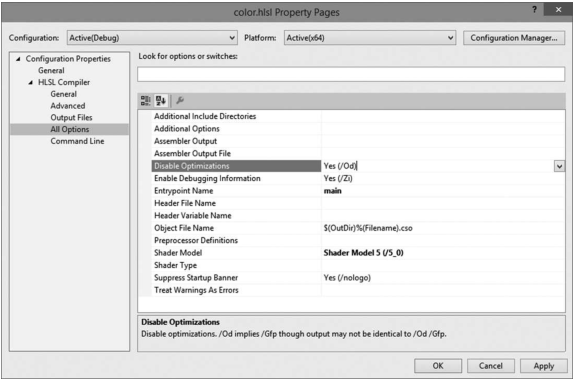
\includegraphics[width=\textwidth]{6-6}
    \centering
    \caption{添加一个自定义编译工具到项目中}
    \label{fig:6-6}
\end{figure}

使用VS集成HLSL支持的一个缺点是它只支持每个文件一个着色器程序。 因此,您不能将顶点和像素着色器存储在一个文件中。 此外,有时候我们希望使用不同的预处理器指令编译相同的着色器程序,以获得着色器的不同变体。 同样,这将不可能使用集成VS支持,因为它是每个.hlsl输入一个.cso输出。
\end{flushleft}

\section{光栅化器状态(Rasterizer State)}
\begin{flushleft}
虽然渲染管线的许多部分都是可编程的,但某些部分只能配置。 由D3D12\_RASTERIZER\_DESC结构表示的光栅化器状态组用于配置渲染管线的光栅化阶段:\\
\begin{lstlisting}
typedef struct D3D12_RASTERIZER_DESC
{
    D3D12_FILL_MODE FillMode;   // Default: D3D12_FILL_SOLID
    D3D12_CULL_MODE CullMode;   // Default: D3D12_CULL_BACK
    BOOL FrontCounterClockwise; // Default: false
    INT DepthBias;              // Default: 0
    FLOAT DepthBiasClamp;       // Default: 0.0f
    FLOAT SlopeScaledDepthBias; // Default: 0.0f
    BOOL DepthClipEnable;       // Default: true
    BOOL ScissorEnable;         // Default: false
    BOOL MultisampleEnable;     // Default: false
    BOOL AntialiasedLineEnable; // Default: false
    UINT ForcedSampleCount;     // Default: 0

    // Default: D3D12_CONSERVATIVE_RASTERIZATION_MODE_OFF
    D3D12_CONSERVATIVE_RASTERIZATION_MODE ConservativeRaster;
} D3D12_RASTERIZER_DESC;
\end{lstlisting}
这些成员大多数是高级选项或不经常使用;详细描述请参阅SDK文档。我们在这里只描述四个。\\
~\\
1.FillMode: 指定 D3D12\_FILL\_WIREFRAME 进行线框渲染或 D3D12\_FILL\_SOLID 用于实体渲染。固体渲染是默认的。\\
2.CullMode: 指定 D3D12\_CULL\_NONE 禁用剔除,D3D12\_CULL\_BACK 剔除背向三角形,或 D3D12\_CULL\_FRONT 剔除前向三角形。 背面三角形默认为剔除。\\
3.FrontCounterClockwise: 如果希望顺时针(相对于相机)顺时针排列的三角形被视为正面,并且逆时针(相对于相机)排列的三角形被视为背面,则指定false。 如果您希望将逆时针(相对于相机)排列的三角形视为正面,并将顺时针(相对于相机)排列的三角形视为背面,请指定true。 此状态默认为false。\\
4.ScissorEnable: 指定true以启用裁剪测试(第4.3.10节),如果为false则禁用它。 默认值是false。\\
~\\
以下代码表示如何创建打开线框模式并禁用背面剔除的栅格化状态:\\
\begin{lstlisting}
CD3DX12_RASTERIZER_DESC rsDesc(D3D12_DEFAULT);
rsDesc.FillMode = D3D12_FILL_WIREFRAME;
rsDesc.CullMode = D3D12_CULL_MODE;
\end{lstlisting}
CD3DX12\_RASTERIZER\_DESC 是一个便捷类,它扩展了 D3D12\_RASTERIZER\_DESC 并添加了一些辅助构造函数。 特别是,它有一个构造函数,它接受一个类型为 CD3D12\_DEFAULT 的对象,该对象只是一个用于重载的虚拟类型,用于将光栅化器状态成员初始化为默认值。CD3D12\_DEFAULT 和 D3D12\_DEFAULT 定义如下:\\
\begin{lstlisting}
struct CD3D12_DEFAULT {};
extern const DECLSPEC_SELECTANY CD3D12_DEFAULT D3D12_DEFAULT;
\end{lstlisting}
几个 Direct3D 便利类会使用 D3D12\_DEFAULT。
\end{flushleft}

\section{管道状态对象(Pipeline State Object)}
\begin{flushleft}
我们已经展示了如何描述输入布局描述,如何创建顶点和像素着色器,以及如何配置光栅器状态组。 但是,我们尚未显示如何将这些对象绑定到图形管道以供实际使用。 控制图形管道状态的大多数对象都被指定为一个称为管道状态对象(PSO)的聚合,它由 ID3D12PipelineState 接口表示。 为了创建一个PSO,我们首先通过填写一个D3D12\_GRAPHICS\_PIPELINE\_STATE\_DESC实例来描述它:\\
\end{flushleft}
\begin{lstlisting}
typedef struct D3D12_GRAPHICS_PIPELINE_STATE_DESC
{
    ID3D12RootSignature *pRootSignature;
    D3D12_SHADER_BYTECODE VS;
    D3D12_SHADER_BYTECODE PS;
    D3D12_SHADER_BYTECODE DS;
    D3D12_SHADER_BYTECODE HS;
    D3D12_SHADER_BYTECODE GS;
    D3D12_STREAM_OUTPUT_DESC StreamOutput;
    D3D12_BLEND_DESC BlendState;
    UINT SampleMask;
    D3D12_RASTERIZER_DESC RasterizerState;
    D3D12_DEPTH_STENCIL_DESC DepthStencilState;
    D3D12_INPUT_LAYOUT_DESC InputLayout;
    D3D12_PRIMITIVE_TOPOLOGY_TYPE PrimitiveTopologyType;
    UINT NumRenderTargets;
    DXGI_FORMAT RTVFormats[8];
    DXGI_FORMAT DSVFormat;
    DXGI_SAMPLE_DESC SampleDesc;
} D3D12_GRAPHICS_PIPELINE_STATE_DESC;
\end{lstlisting}
\begin{flushleft}
1.pRootSignature: 指向与此PSO绑定的根签名的指针。根签名必须与此PSO指定的着色器兼容。\\
2.VS: 要绑定的顶点着色器。 这由 D3D12\_SHADER\_BYTECODE 结构指定,该结构是指向编译的字节码数据的指针,以及字节码数据的大小(以字节为单位)。\\
3.PS: 要绑定的像素着色器。\\
4.DS: 要绑定的域着色器。(我们将在之后的章节讨论)\\
5.HS: 要绑定的外壳着色器。(我们将在之后的章节讨论)\\
6.GS: 要绑定的几何着色器。(我们将在之后的章节讨论)\\
7.StreamOutput: 用于称(流出)stream-out的高级技术。现在我们只是把这个领域归零(zero-out)。\\
8.BlendState: 指定配置混合的混合状态。 我们将在后面的章节中讨论这个状态组; 现在,指定默认 CD3DX12\_BLEND\_DESC(D3D12\_DEFAULT)。\\
9.SampleMask: 多重采样可能需要多达32个样本。 该32位整数值用于启用/禁用采样。 例如,如果关闭第5位,则第5个采样不会被采用。 当然,如果您实际使用至少5个采样的多重采样,则禁用第5个采样只会产生任何结果。 如果应用程序使用单个采样,则只有该参数的第一位很重要。 通常使用默认的0xffffffff,这不会禁用任何样本。\\
10.RasterizerState: 指定配置光栅化器的光栅化状态。\\
11.DepthStencilState: 指定配置深度/模板测试的深度/模板状态。 我们将在后面的章节中讨论这个状态组; 现在,指定默认CD3DX12\_DEPTH\_STENCIL\_DESC(D3D12\_DEFAULT)。
12.InputLayout: 输入布局描述,它只是D3D12\_INPUT\_ELEMENT\_DESC元素的一个数组,以及数组中的元素数。\\
\begin{lstlisting}
typedef struct D3D12_INPUT_LAYOUT_DESC
{
    const D3D12_INPUT_ELEMENT_DESC *pInputElementDescs;
    UINT NumElements;
} D3D12_INPUT_LAYOUT_DESC;
\end{lstlisting}
13.PrimitiveTopologyType: 指定原始拓扑类型。\\
\begin{lstlisting}
typedef enum D3D12_PRIMITIVE_TOPOLOGY_TYPE
{
    D3D12_PRIMITIVE_TOPOLOGY_TYPE_UNDEFINED = 0,
    D3D12_PRIMITIVE_TOPOLOGY_TYPE_POINT = 1,
    D3D12_PRIMITIVE_TOPOLOGY_TYPE_LINE = 2,
    D3D12_PRIMITIVE_TOPOLOGY_TYPE_TRIANGLE = 3,
    D3D12_PRIMITIVE_TOPOLOGY_TYPE_PATCH = 4
} D3D12_PRIMITIVE_TOPOLOGY_TYPE;
\end{lstlisting}
14.NumRenderTargets: 我们正在同时使用的渲染目标的数量。\\
15.RTVFormats: 呈现目标格式。 这是一个支持同时写入多个渲染目标的数组。 这应该与我们使用PSO的渲染目标的设置相匹配。\\
16.DSVFormat: 深度/模板缓冲区的格式。 这应该与我们使用PSO的深度/模板缓冲区的设置匹配。\\
17.SampleDesc: 介绍多重采样计数和质量级别。 这应该与我们正在使用的渲染目标的设置相匹配。\\
~\\
在我们填写完一个 D3D12\_GRAPHICS\_PIPELINE\_STATE\_DESC 实例后,我们使用 ID3D12Device::CreateGraphicsPipelineState 方法创建一个 ID3D12PipelineState 对象:\\
\begin{lstlisting}
ComPtr<ID3D12RootSignature> mRootSignature;
std::vector<D3D12_INPUT_ELEMENT_DESC> mInputLayout;
ComPtr<ID3DBlob> mvsByteCode;
ComPtr<ID3DBlob> mpsByteCode;
...
D3D12_GRAPHICS_PIPELINE_STATE_DESC psoDesc;
ZeroMemory(&psoDesc, 
           sizeof(D3D12_GRAPHICS_PIPELINE_STATE_DESC));
psoDesc.InputLayout = {
    mInputLayout.data(),
   (UINT)mInputLayout.size()
};
psoDesc.pRootSignature = mRootSignature.Get();
psoDesc.VS = {
    reinterpret_cast<BYTE*>(mvsByteCode->GetBufferPointer()),
    mvsByteCode->GetBufferSize()
};
psoDesc.PS = {
    reinterpret_cast<BYTE*>(mpsByteCode->GetBufferPointer()),
    mpsByteCode->GetBufferSize()
};
psoDesc.RasterizerState = CD3D12_RASTERIZER_DESC(D3D12_DEFAULT);
psoDesc.BlendState = CD3D12_BLEND_DESC(D3D12_DEFAULT);
psoDesc.DepthStencilState = CD3D12_DEPTH_STENCIL_DESC(D3D12_DEFAULT);
psoDesc.SampleMask = UINT_MAX;
psoDesc.PrimitiveTopologyType = D3D12_PRIMITIVE_TOPOLOGY_TYPE_TRIANGLE;
psoDesc.NumRenderTargets = 1;
psoDesc.RTVFormats[0] = mBackBufferFormat;
psoDesc.SampleDesc.Count = m4xMsaaState ? 4 : 1;
psoDesc.SampleDesc.Quality = m4xMsaaState ? (m4xMsaaQuality - 1) : 0;
psoDesc.DSVFormat = mDepthStencilFormat;

ComPtr<ID3D12PipelineState> mPSO;
md3dDevice->CreateGraphicsPipelineState(&psoDesc,IID_PPV_ARGS(&mPSO)));
\end{lstlisting}
上述代码用 ID3D12PipelineState 对象聚合(aggregate)了很多状态,出于性能考虑,我们指定所有这些对象都作为一个聚合传递到图形管线中。通过将它们作为聚合,Direct3D可以验证所有状态是否兼容,驱动程序可以预先生成所有代码以编写硬件状态。在Direct3D 11状态模型中,这些渲染状态片段是分开设置的。但是,各个状态是相关的; 如果一个状态被改变,它可能会另外要求驱动程序重新编程硬件以获取另一个依赖状态。由于配置流水线的许多状态会被改变,所以硬件的状态可能会被多次重新编写。为了避免这种情况,驱动程序通常推迟对硬件状态进行编写,直到在整个管道状态将被知道时发出绘制调用。但是这种延期需要驱动在运行时进行额外的记录工作; 它需要跟踪哪些状态发生了变化,然后生成代码以在运行时对硬件状态进行编程。 在新的Direct3D 12模型中,驱动程序可以在初始化时生成编程流水线状态所需的所有代码,因为我们将大部分流水线状态指定为聚合。\\
~\\
NOTICE:由于PSO验证和创建可能非常耗时,PSO应该在初始化时生成。 对此的一个例外可能是在运行时第一次引用PSO时创建PSO; 然后将其存储在哈希表等集合中,以便将来可以快速获取以供将来使用。\\
~\\
并非所有渲染状态都封装在PSO中。 一些像视口和裁剪矩形的状态是独立于PSO的。 这种状态可以独立于另一个管道状态而有效地设置,因此将它们包含在PSO中没有任何优势。\\
Direct3D基本上是一个状态机。 在我们改变它们之前,事物会保持现状。 如果您正在绘制的某些对象使用一个PSO,并且您正在绘制的其他对象需要不同的PSO,那么您需要像这样构造代码:\\
\begin{lstlisting}
// Reset specifies initial PSO.
mCommandList->Reset(mDirectCmdListAlloc.Get(), mPSO1.Get());
/*...draw objects using PSO 1...*/
// Change PSO
mCommandList->SetPipelineState(mPSO2.Get());
/*...draw objects using PSO 2...*/
// Change PSO
mCommandList->SetPipelineState(mPSO3.Get());
/*...draw objects using PSO 3...*/
\end{lstlisting}
换句话说,当PSO绑定到命令列表时,它不会改变,直到你覆盖它(或命令列表被重置)。\\
~\\
NOTICE: 出于性能考虑,PSO状态变化应该保持在最小。 一起绘制可以使用相同PSO的所有对象。 不要更改每次绘制调用的PSO!
\end{flushleft}

\section{几何工具结构体(Geometry Helper Structure)}
\begin{flushleft}
创建一个将顶点和索引缓冲区组合在一起以定义一组几何体的结构会很有帮助。 另外,这种结构可以保留顶点和索引数据的系统内存支持,以便可以由CPU读取。 CPU将需要访问几何数据以进行拾取和碰撞检测等操作。 另外,结构缓存顶点和索引缓冲区的重要属性,如格式和碰撞,并提供返回视图到缓冲区的方法。 每当我们定义一个几何体块时,我们在整本书中使用下面的MeshGeometry(在d3dUtil.h中定义)结构。\\
\begin{lstlisting}
// Defines a subrange of geometry in a MeshGeometry. This is for when
// multiple geometries are stored in one vertex and index buffer. It
// provides the offsets and data needed to draw a subset of geometry
// stores in the vertex and index buffers so that we can implement the
// technique described by Figure \ref{fig:6-3}.
struct SubmeshGeometry
{
    UINT IndexCount = 0;
    UINT StartIndexLocation = 0;
    INT  BaseVertexLocation = 0;

    // Bounding box of the geometry defined by this submesh.
    // This is used in later chapters of the book.
    DirectX::BoundingBox Bounds;
};

struct MeshGeometry
{
    // Give it a name so we can look it up by name.
    std::string Name;

    // System memory copies. Use Blobs because the vertex/index format can
    // be generic.
    // It is up to the client to cast appropriately.
    Microsoft::WRL::ComPtr<ID3DBlob> VertexBufferCPU = nullptr;
    Microsoft::WRL::ComPtr<ID3DBlob> IndexBufferCPU = nullptr;

    Microsoft::WRL::ComPtr<ID3D12Resource> VertexBufferGPU = nullptr;
    Microsoft::WRL::ComPtr<ID3D12Resource> IndexBufferGPU = nullptr;
    
    Microsoft::WRL::ComPtr<ID3D12Resource> VertexBufferUploader = nullptr;
    Microsoft::WRL::ComPtr<ID3D12Resource> IndexBufferUploader = nullptr;
    
    // Data about the buffers
    UINT VertexByteStride = 0;
    UINT VertexBufferByteSize = 0;
    DXGI_FORMAT IndexFormat = DXGI_FORMAT_R16_UINT;
    UINT IndexBufferByteSize = 0;
    
    // A MeshGeometry may store multiple geometries in one vertex/index
    // buffer.
    // Use this container to define the Submesh geometries so we can draw
    // the Submeshes individually.
    std::unordered_map<std::string, SubmeshGeometry> DrawArgs;
    
    D3D12_VERTEX_BUFFER_VIEW VertexBufferView() const
        D3D12_VERTEX_BUFFER_VIEW vbv;
    {
        vbv.BufferLocation = VertexBufferGPU->GetGPUVirtualAddress();
        vbv.StrideInBytes = VertexByteStride;
        vbv.SizeInBytes = VertexBufferByteSize;

        return vbv;
    }
    
    D3D12_INDEX_BUFFER_VIEW IndexBufferView() const
    {
        D3D12_INDEX_BUFFER_VIEW ibv;
        ibv.BufferLocation = IndexBufferGPU->GetGPUVirtualAddress();
        ibv.Format = IndexFormat;
        ibv.SizeInBytes = IndexBufferByteSize;

        return ibv;
    }
    
    // We can free this memory after we finish upload to the GPU.
    void DisposeUploaders()
    {
       VertexBufferUploader = nullptr;
       IndexBufferUploader = nullptr;
    }
};
\end{lstlisting}
\end{flushleft}

\section{BOX DEMO}
\begin{flushleft}
最后,我们已经有足够的能力去做出渲染一个彩箱(彩色立方体)的DEMO。这个例子基本上将我们在本章中讨论过的所有内容都放到了一个程序中。 读者应该研究代码并参考本章前面的部分,直到理解每一行。程序所使用的 Shaders\\color.hlsl, 见 6.5 节(像素着色器例子)末尾。
\end{flushleft}
\begin{lstlisting}
//**************************************************************************
// BoxApp.cpp by Frank Luna (C) 2015 All Rights Reserved.
//
// Shows how to draw a box in Direct3D 12.
//
// Controls:
//   Hold the left mouse button down and move the mouse to rotate.
//   Hold the right mouse button down and move the mouse to zoom in and out.
//**************************************************************************

#include "../../Common/d3dApp.h"
#include "../../Common/MathHelper.h"
#include "../../Common/UploadBuffer.h"

using Microsoft::WRL::ComPtr;
using namespace DirectX;
using namespace DirectX::PackedVector;

struct Vertex
{
    XMFLOAT3 Pos;
    XMFLOAT4 Color;
};

struct ObjectConstants
{
    XMFLOAT4X4 WorldViewProj = MathHelper::Identity4x4();
};

class BoxApp : public D3DApp
{
public:
    BoxApp(HINSTANCE hInstance);
    BoxApp(const BoxApp& rhs) = delete;
    BoxApp& operator=(const BoxApp& rhs) = delete;
    ~BoxApp();

    virtual bool Initialize()override;

private:
    virtual void OnResize()override;
    virtual void Update(const GameTimer& gt)override;
    virtual void Draw(const GameTimer& gt)override;

    virtual void OnMouseDown(WPARAM btnState, int x, int y)override;
    virtual void OnMouseUp(WPARAM btnState, int x, int y)override;
    virtual void OnMouseMove(WPARAM btnState, int x, int y)override;

    void BuildDescriptorHeaps();
    void BuildConstantBuffers();
    void BuildRootSignature();
    void BuildShadersAndInputLayout();
    void BuildBoxGeometry();
    void BuildPSO();

private:
    
    ComPtr<ID3D12RootSignature> mRootSignature = nullptr;
    ComPtr<ID3D12DescriptorHeap> mCbvHeap = nullptr;

    std::unique_ptr<UploadBuffer<ObjectConstants>> mObjectCB = nullptr;

    std::unique_ptr<MeshGeometry> mBoxGeo = nullptr;

    ComPtr<ID3DBlob> mvsByteCode = nullptr;
    ComPtr<ID3DBlob> mpsByteCode = nullptr;

    std::vector<D3D12_INPUT_ELEMENT_DESC> mInputLayout;

    ComPtr<ID3D12PipelineState> mPSO = nullptr;

    XMFLOAT4X4 mWorld = MathHelper::Identity4x4();
    XMFLOAT4X4 mView = MathHelper::Identity4x4();
    XMFLOAT4X4 mProj = MathHelper::Identity4x4();

    float mTheta = 1.5f*XM_PI;
    float mPhi = XM_PIDIV4;
    float mRadius = 5.0f;

    POINT mLastMousePos;
};

int WINAPI WinMain(HINSTANCE hInstance, HINSTANCE prevInstance,
                   PSTR cmdLine, int showCmd)
{
    // Enable run-time memory check for debug builds.
#if defined(DEBUG) | defined(_DEBUG)
    _CrtSetDbgFlag( _CRTDBG_ALLOC_MEM_DF | _CRTDBG_LEAK_CHECK_DF );
#endif

    try
    {
        BoxApp theApp(hInstance);
        if(!theApp.Initialize())
            return 0;

        return theApp.Run();
    }
    catch(DxException& e)
    {
        MessageBox(nullptr, e.ToString().c_str(), L"HR Failed", MB_OK);
        return 0;
    }
}

BoxApp::BoxApp(HINSTANCE hInstance)
: D3DApp(hInstance) 
{
}

BoxApp::~BoxApp()
{
}

bool BoxApp::Initialize()
{
    if(!D3DApp::Initialize())
        return false;
        
    // Reset the command list to prep for initialization commands.
    ThrowIfFailed(mCommandList->Reset(mDirectCmdListAlloc.Get(), nullptr));
 
    BuildDescriptorHeaps();
    BuildConstantBuffers();
    BuildRootSignature();
    BuildShadersAndInputLayout();
    BuildBoxGeometry();
    BuildPSO();

    // Execute the initialization commands.
    ThrowIfFailed(mCommandList->Close());
    ID3D12CommandList* cmdsLists[] = { mCommandList.Get() };
    mCommandQueue->ExecuteCommandLists(_countof(cmdsLists), cmdsLists);

    // Wait until initialization is complete.
    FlushCommandQueue();

    return true;
}

void BoxApp::OnResize()
{
    D3DApp::OnResize();

    // The window resized, so update the aspect ratio 
    // and recompute the projection matrix.
    XMMATRIX P = XMMatrixPerspectiveFovLH(
                     0.25f*MathHelper::Pi, 
                     AspectRatio(), 
                     1.0f, 1000.0f);
    XMStoreFloat4x4(&mProj, P);
}

void BoxApp::Update(const GameTimer& gt)
{
    // Convert Spherical to Cartesian coordinates.
    float x = mRadius*sinf(mPhi)*cosf(mTheta);
    float z = mRadius*sinf(mPhi)*sinf(mTheta);
    float y = mRadius*cosf(mPhi);

    // Build the view matrix.
    XMVECTOR pos = XMVectorSet(x, y, z, 1.0f);
    XMVECTOR target = XMVectorZero();
    XMVECTOR up = XMVectorSet(0.0f, 1.0f, 0.0f, 0.0f);

    XMMATRIX view = XMMatrixLookAtLH(pos, target, up);
    XMStoreFloat4x4(&mView, view);

    XMMATRIX world = XMLoadFloat4x4(&mWorld);
    XMMATRIX proj = XMLoadFloat4x4(&mProj);
    XMMATRIX worldViewProj = world*view*proj;

    // Update the constant buffer with 
    // the latest worldViewProj matrix.
    ObjectConstants objConstants;
    XMStoreFloat4x4(&objConstants.WorldViewProj, 
                    XMMatrixTranspose(worldViewProj));
    mObjectCB->CopyData(0, objConstants);
}

void BoxApp::Draw(const GameTimer& gt)
{
    // Reuse the memory associated with command recording.
    // We can only reset when the associated command lists 
    // have finished execution on the GPU.
    ThrowIfFailed(mDirectCmdListAlloc->Reset());

    // A command list can be reset after it has 
    // been added to the command queue via ExecuteCommandList.
    // Reusing the command list reuses memory.
    ThrowIfFailed(mCommandList->Reset(mDirectCmdListAlloc.Get(), 
                                      mPSO.Get()));

    mCommandList->RSSetViewports(1, &mScreenViewport);
    mCommandList->RSSetScissorRects(1, &mScissorRect);

    // Indicate a state transition on the resource usage.
    mCommandList->ResourceBarrier(1, 
                 &CD3DX12_RESOURCE_BARRIER::Transition(
                      CurrentBackBuffer(),
                      D3D12_RESOURCE_STATE_PRESENT, 
                      D3D12_RESOURCE_STATE_RENDER_TARGET));

    // Clear the back buffer and depth buffer.
    mCommandList->ClearRenderTargetView(
                      CurrentBackBufferView(), 
                      Colors::LightSteelBlue, 
                      0, nullptr);
    mCommandList->ClearDepthStencilView(
                      DepthStencilView(), 
                      D3D12_CLEAR_FLAG_DEPTH | D3D12_CLEAR_FLAG_STENCIL, 
                      1.0f, 0, 0, nullptr);
    
    // Specify the buffers we are going to render to.
    mCommandList->OMSetRenderTargets(1, 
                        &CurrentBackBufferView(), 
                        true, 
                        &DepthStencilView());

    ID3D12DescriptorHeap* descriptorHeaps[] = { mCbvHeap.Get() };
    mCommandList->SetDescriptorHeaps(_countof(descriptorHeaps), 
                                     descriptorHeaps);

    mCommandList->SetGraphicsRootSignature(mRootSignature.Get());

    mCommandList->IASetVertexBuffers(
                      0, 1, &mBoxGeo->VertexBufferView());
    mCommandList->IASetIndexBuffer(
                      &mBoxGeo->IndexBufferView());
    mCommandList->IASetPrimitiveTopology(
                      D3D11_PRIMITIVE_TOPOLOGY_TRIANGLELIST);
    
    mCommandList->SetGraphicsRootDescriptorTable(0, 
                      mCbvHeap->GetGPUDescriptorHandleForHeapStart());

    mCommandList->DrawIndexedInstanced(
        mBoxGeo->DrawArgs["box"].IndexCount, 
        1, 0, 0, 0);
    
    // Indicate a state transition on the resource usage.
    mCommandList->ResourceBarrier(1, 
                 &CD3DX12_RESOURCE_BARRIER::Transition(
                      CurrentBackBuffer(),
                      D3D12_RESOURCE_STATE_RENDER_TARGET, 
                      D3D12_RESOURCE_STATE_PRESENT));

    // Done recording commands.
    ThrowIfFailed(mCommandList->Close());
 
    // Add the command list to the queue for execution.
    ID3D12CommandList* cmdsLists[] = { mCommandList.Get() };
    mCommandQueue->ExecuteCommandLists(_countof(cmdsLists), cmdsLists);
    
    // swap the back and front buffers
    ThrowIfFailed(mSwapChain->Present(0, 0));
    mCurrBackBuffer = (mCurrBackBuffer + 1) % SwapChainBufferCount;

    // Wait until frame commands are complete.  
    // This waiting is inefficient and is
    // done for simplicity.  Later we will 
    // show how to organize our rendering code
    // so we do not have to wait per frame.
    FlushCommandQueue();
}

void BoxApp::OnMouseDown(WPARAM btnState, int x, int y)
{
    mLastMousePos.x = x;
    mLastMousePos.y = y;

    SetCapture(mhMainWnd);
}

void BoxApp::OnMouseUp(WPARAM btnState, int x, int y)
{
    ReleaseCapture();
}

void BoxApp::OnMouseMove(WPARAM btnState, int x, int y)
{
    if((btnState & MK_LBUTTON) != 0)
    {
        // Make each pixel correspond to a quarter of a degree.
        float dx = XMConvertToRadians(
                       0.25f*static_cast<float>(x - mLastMousePos.x));
        float dy = XMConvertToRadians(
                       0.25f*static_cast<float>(y - mLastMousePos.y));

        // Update angles based on input to orbit camera around box.
        mTheta += dx;
        mPhi += dy;

        // Restrict the angle mPhi.
        mPhi = MathHelper::Clamp(mPhi, 0.1f, MathHelper::Pi - 0.1f);
    }
    else if((btnState & MK_RBUTTON) != 0)
    {
        // Make each pixel correspond to 0.005 unit in the scene.
        float dx = 0.005f*static_cast<float>(x - mLastMousePos.x);
        float dy = 0.005f*static_cast<float>(y - mLastMousePos.y);

        // Update the camera radius based on input.
        mRadius += dx - dy;

        // Restrict the radius.
        mRadius = MathHelper::Clamp(mRadius, 3.0f, 15.0f);
    }

    mLastMousePos.x = x;
    mLastMousePos.y = y;
}

void BoxApp::BuildDescriptorHeaps()
{
    D3D12_DESCRIPTOR_HEAP_DESC cbvHeapDesc;
    cbvHeapDesc.NumDescriptors = 1;
    cbvHeapDesc.Type = D3D12_DESCRIPTOR_HEAP_TYPE_CBV_SRV_UAV;
    cbvHeapDesc.Flags = D3D12_DESCRIPTOR_HEAP_FLAG_SHADER_VISIBLE;
    cbvHeapDesc.NodeMask = 0;
    ThrowIfFailed(md3dDevice->CreateDescriptorHeap(&cbvHeapDesc,
        IID_PPV_ARGS(&mCbvHeap)));
}

void BoxApp::BuildConstantBuffers()
{
    mObjectCB = std::make_unique<UploadBuffer<ObjectConstants>>(
                    md3dDevice.Get(), 1, true);

    UINT objCBByteSize = d3dUtil::CalcConstantBufferByteSize(
                             sizeof(ObjectConstants));

    D3D12_GPU_VIRTUAL_ADDRESS cbAddress = mObjectCB->Resource()
                                              ->GetGPUVirtualAddress();

    // Offset to the ith object constant buffer in the buffer.
    int boxCBufIndex = 0;
    cbAddress += boxCBufIndex*objCBByteSize;

    D3D12_CONSTANT_BUFFER_VIEW_DESC cbvDesc;
    cbvDesc.BufferLocation = cbAddress;
    cbvDesc.SizeInBytes = d3dUtil::CalcConstantBufferByteSize(
                              sizeof(ObjectConstants));

    md3dDevice->CreateConstantBufferView(
        &cbvDesc,
        mCbvHeap->GetCPUDescriptorHandleForHeapStart());
}

void BoxApp::BuildRootSignature()
{
    // Shader programs typically require resources as input 
    // (constant buffers, textures, samplers).  
    // The root signature defines the resources the shader
    // programs expect.  If we think of the shader programs 
    // as a function, and the input resources as function parameters,
    // then the root signature can be thought of as defining
    // the function signature.  

    // Root parameter can be a table, root descriptor or root constants.
    CD3DX12_ROOT_PARAMETER slotRootParameter[1];

    // Create a single descriptor table of CBVs.
    CD3DX12_DESCRIPTOR_RANGE cbvTable;
    cbvTable.Init(D3D12_DESCRIPTOR_RANGE_TYPE_CBV, 1, 0);
    slotRootParameter[0].InitAsDescriptorTable(1, &cbvTable);

    // A root signature is an array of root parameters.
    CD3DX12_ROOT_SIGNATURE_DESC rootSigDesc(1, slotRootParameter, 
                                            0, nullptr, 
        D3D12_ROOT_SIGNATURE_FLAG_ALLOW_INPUT_ASSEMBLER_INPUT_LAYOUT);

    // create a root signature with a single slot
    // which points to a descriptor range consisting 
    // of a single constant buffer
    ComPtr<ID3DBlob> serializedRootSig = nullptr;
    ComPtr<ID3DBlob> errorBlob = nullptr;
    HRESULT hr = D3D12SerializeRootSignature(&rootSigDesc, 
                     D3D_ROOT_SIGNATURE_VERSION_1,
                     serializedRootSig.GetAddressOf(), 
                     errorBlob.GetAddressOf());

    if(errorBlob != nullptr)
    {
        ::OutputDebugStringA((char*)errorBlob->GetBufferPointer());
    }
    ThrowIfFailed(hr);

    ThrowIfFailed(md3dDevice->CreateRootSignature(
        0,
        serializedRootSig->GetBufferPointer(),
        serializedRootSig->GetBufferSize(),
        IID_PPV_ARGS(&mRootSignature)));
}

void BoxApp::BuildShadersAndInputLayout()
{
    HRESULT hr = S_OK;
    
    mvsByteCode = d3dUtil::CompileShader(L"Shaders\\color.hlsl", 
                      nullptr, "VS", "vs_5_0");
    mpsByteCode = d3dUtil::CompileShader(L"Shaders\\color.hlsl", 
                      nullptr, "PS", "ps_5_0");

    mInputLayout =
    {
        { "POSITION", 0, DXGI_FORMAT_R32G32B32_FLOAT, 0, 0, 
                      D3D12_INPUT_CLASSIFICATION_PER_VERTEX_DATA, 0 },
        { "COLOR",    0, DXGI_FORMAT_R32G32B32A32_FLOAT, 0, 12, 
                      D3D12_INPUT_CLASSIFICATION_PER_VERTEX_DATA, 0 }
    };
}

void BoxApp::BuildBoxGeometry()
{
    std::array<Vertex, 8> vertices =
    {
        Vertex({ XMFLOAT3(-1.0f, -1.0f, -1.0f), XMFLOAT4(Colors::White) }),
        Vertex({ XMFLOAT3(-1.0f, +1.0f, -1.0f), XMFLOAT4(Colors::Black) }),
        Vertex({ XMFLOAT3(+1.0f, +1.0f, -1.0f), XMFLOAT4(Colors::Red) }),
        Vertex({ XMFLOAT3(+1.0f, -1.0f, -1.0f), XMFLOAT4(Colors::Green) }),
        Vertex({ XMFLOAT3(-1.0f, -1.0f, +1.0f), XMFLOAT4(Colors::Blue) }),
        Vertex({ XMFLOAT3(-1.0f, +1.0f, +1.0f), XMFLOAT4(Colors::Yellow) }),
        Vertex({ XMFLOAT3(+1.0f, +1.0f, +1.0f), XMFLOAT4(Colors::Cyan) }),
        Vertex({ XMFLOAT3(+1.0f, -1.0f, +1.0f), XMFLOAT4(Colors::Magenta) })
    };

    std::array<std::uint16_t, 36> indices =
    {
        // front face
        0, 1, 2,
        0, 2, 3,

        // back face
        4, 6, 5,
        4, 7, 6,

        // left face
        4, 5, 1,
        4, 1, 0,

        // right face
        3, 2, 6,
        3, 6, 7,

        // top face
        1, 5, 6,
        1, 6, 2,

        // bottom face
        4, 0, 3,
        4, 3, 7
    };

    const UINT vbByteSize = (UINT)vertices.size() * sizeof(Vertex);
    const UINT ibByteSize = (UINT)indices.size() * sizeof(std::uint16_t);

    mBoxGeo = std::make_unique<MeshGeometry>();
    mBoxGeo->Name = "boxGeo";

    ThrowIfFailed(D3DCreateBlob(vbByteSize, 
                                &mBoxGeo->VertexBufferCPU));
    CopyMemory(mBoxGeo->VertexBufferCPU->GetBufferPointer(),
               vertices.data(), vbByteSize);

    ThrowIfFailed(D3DCreateBlob(ibByteSize, 
                                &mBoxGeo->IndexBufferCPU));
    CopyMemory(mBoxGeo->IndexBufferCPU->GetBufferPointer(), 
               indices.data(), ibByteSize);

    mBoxGeo->VertexBufferGPU = d3dUtil::CreateDefaultBuffer(
                                   md3dDevice.Get(),
                                   mCommandList.Get(), 
                                   vertices.data(), 
                                   vbByteSize, 
                                   mBoxGeo->VertexBufferUploader);

    mBoxGeo->IndexBufferGPU = d3dUtil::CreateDefaultBuffer(
                                  md3dDevice.Get(),
                                  mCommandList.Get(),
                                  indices.data(), 
                                  ibByteSize, 
                                  mBoxGeo->IndexBufferUploader);

    mBoxGeo->VertexByteStride = sizeof(Vertex);
    mBoxGeo->VertexBufferByteSize = vbByteSize;
    mBoxGeo->IndexFormat = DXGI_FORMAT_R16_UINT;
    mBoxGeo->IndexBufferByteSize = ibByteSize;

    SubmeshGeometry submesh;
    submesh.IndexCount = (UINT)indices.size();
    submesh.StartIndexLocation = 0;
    submesh.BaseVertexLocation = 0;

    mBoxGeo->DrawArgs["box"] = submesh;
}

void BoxApp::BuildPSO()
{
    D3D12_GRAPHICS_PIPELINE_STATE_DESC psoDesc;
    ZeroMemory(&psoDesc, sizeof(D3D12_GRAPHICS_PIPELINE_STATE_DESC));
    psoDesc.InputLayout = { mInputLayout.data(), 
                            (UINT)mInputLayout.size() };
    psoDesc.pRootSignature = mRootSignature.Get();
    psoDesc.VS = 
    { 
        reinterpret_cast<BYTE*>(mvsByteCode->GetBufferPointer()), 
        mvsByteCode->GetBufferSize() 
    };
    psoDesc.PS = 
    { 
        reinterpret_cast<BYTE*>(mpsByteCode->GetBufferPointer()), 
        mpsByteCode->GetBufferSize() 
    };
    psoDesc.RasterizerState = CD3DX12_RASTERIZER_DESC(D3D12_DEFAULT);
    psoDesc.BlendState = CD3DX12_BLEND_DESC(D3D12_DEFAULT);
    psoDesc.DepthStencilState = CD3DX12_DEPTH_STENCIL_DESC(D3D12_DEFAULT);
    psoDesc.SampleMask = UINT_MAX;
    psoDesc.PrimitiveTopologyType = D3D12_PRIMITIVE_TOPOLOGY_TYPE_TRIANGLE;
    psoDesc.NumRenderTargets = 1;
    psoDesc.RTVFormats[0] = mBackBufferFormat;
    psoDesc.SampleDesc.Count = m4xMsaaState ? 4 : 1;
    psoDesc.SampleDesc.Quality = m4xMsaaState ? (m4xMsaaQuality - 1) : 0;
    psoDesc.DSVFormat = mDepthStencilFormat;
    ThrowIfFailed(md3dDevice->CreateGraphicsPipelineState(&psoDesc, 
                                   IID_PPV_ARGS(&mPSO)));
}
\end{lstlisting}
\begin{figure}[h]
	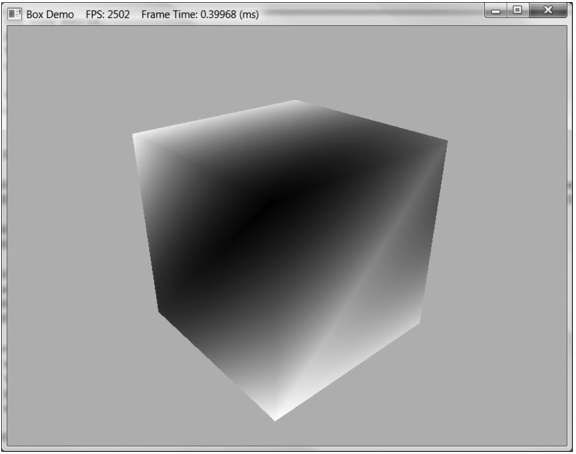
\includegraphics[width=\textwidth]{6-7}
	\centering
	\caption{Box DEMO 截图}
	\label{fig:6-7}
\end{figure}

\section{总结}
TODO:

\section{练习}
%---------- 1 ----------------
\begin{flushleft}
1. 写出下面顶点结构的 D3D12\_INPUT\_ELEMENT\_DESC 数组:
\end{flushleft}
\begin{lstlisting}
struct Vertex
{
    XMFLOAT3 Pos;
    XMFLOAT3 Tangent;
    XMFLOAT3 Normal;
    XMFLOAT2 Tex0;
    XMFLOAT2 Tex1;
    XMCOLOR  Color;
};
\end{lstlisting}

%---------- 2 ----------------
\begin{flushleft}
~\\
2. 重写彩箱DEMO,这次使用 2 个顶点缓冲区(2个输入槽)给管道提供顶点数据。一个缓冲区存储位置元素,另一个存储存储颜色元素。下面给定两个分开的顶点数据结构:\\
\end{flushleft}
\begin{lstlisting}
struct VPosData
{
    XMFLOAT3 Pos;
};

struct VColorData
{
    XMFLOAT4 Color;
};
\end{lstlisting}
\begin{flushleft}
位置元素挂在输入槽0上,颜色元素挂在输入操1上。此外还需注意 D3D12\_INPUT\_ELEMENT\_DESC::AlignedByteOffset 对于两个元素来说都是0;然后使用 ID3D12CommandList::IASetVertexBuffers 方法来将缓冲区绑定到槽0和槽1。然后,Direct3D将使用来自不同输入槽的元素来组合顶点。 这可以用作优化。 例如,在阴影映射算法中,我们需要每帧绘制两次场景:一次从光源的角度(阴影传递),一次从主摄像头的角度(主传递)。 阴影传递仅需要位置数据和纹理坐标(对于经过alpha测试的几何体)。 因此我们可以将顶点数据分成两个槽:一个槽包含位置和纹理坐标,另一个槽包含其他顶点属性(例如,法线和切线矢量)。 现在我们可以轻松地仅在阴影传递所需的顶点数据中流动(位置和纹理坐标),从而为阴影传递节省数据带宽。 主渲染过程将使用两个顶点输入槽来获取所需的所有顶点数据。 为了提高性能,建议最小化用于小于或等于3的小数字的输入槽数。\\
\end{flushleft}

%---------- 3 ----------------
\begin{flushleft}
3. 绘制以下图形:\\
\begin{itemize}
  \item 1. 一个点列表,如图5.13a。
  \item 2. 一个线段条,如图5.13b。
  \item 3. 一个线段列表,如图5.13c。
  \item 4. 一个三角条,如图5.13d。
  \item 5. 一个三角列表,如图5.14a。
\end{itemize}
\end{flushleft}

%---------- 4 ----------------
\begin{flushleft}
4. 构造金字塔的顶点和索引列表,如图\ref{fig:6-8}所示,并绘制它。 将基顶点设为绿色和顶上顶点设为红色。\\
\end{flushleft}
\begin{figure}[h]
    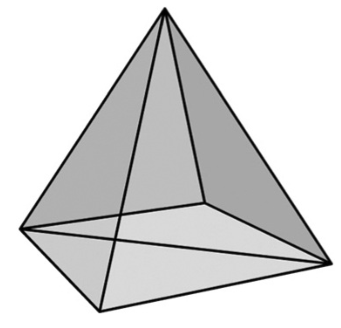
\includegraphics[width=\textwidth]{6-8}
    \centering
    \caption{金字塔三角形}
    \label{fig:6-8}
\end{figure}
%---------- 5 ----------------
\begin{flushleft}
5. 运行“Box” DEMO,并回想一下我们仅在顶点指定颜色。 解释如何为三角形上的每个像素获取像素颜色。
\end{flushleft}


%---------- 6 ----------------
\begin{flushleft}
6. 修改 Box Demo, 在转换为世界空间之前将以下变换应用于顶点着色器中的每个顶点。
\end{flushleft}
\begin{lstlisting}
vin.PosL.xy += 0.5f*sin(vinL.Pos.x)*sin(3.0f*gTime);
vin.PosL.z *= 0.6f + 0.4f*sin(2.0f*gTime);
\end{lstlisting}
\begin{flushleft}
您需要添加一个gTime常量缓冲区变量; 此变量对应于当前的 GameTimer::TotalTime() 值。 使用正弦函数周期性地扭曲顶点来将时间通过顶点动画来展现。
\end{flushleft}

%---------- 7 ----------------
\begin{flushleft}
7. 将箱(box)和金字塔的顶点(练习4)合并到一个大的顶点缓冲区中。 还将框和金字塔的索引合并到一个大索引缓冲区中(但不更新索引值)。 然后使用 ID3D12CommandList::DrawIndexedInstanced 的参数逐个绘制框和金字塔。 使用世界变换矩阵,使框和金字塔在世界空间中不相交。
\end{flushleft}

%---------- 8 ----------------
\begin{flushleft}
8. 通过在线框(wireframe)模式下渲染多维数据集来修改Box演示。
\end{flushleft}

%---------- 9 ----------------
\begin{flushleft}
9. 修改Box演示, 禁用背面剔除(D3D12\_CULL\_NONE); 也尝试剔除正面而不是背面(D3D12\_CULL\_FRONT)。 以线框(wireframe)模式输出结果,以便您可以更轻松地查看差异。
\end{flushleft}

%---------- 10 ----------------
\begin{flushleft}
10. 如果顶点内存很重要,那么从128位颜色值减少到32位颜色值可能是值得的。修改“Box”演示 在顶点结构中使用32位颜色值而不是128位颜色值。 您的顶点结构和相应的顶点输入描述将如下所示:\\
\end{flushleft}
\begin{lstlisting}
struct Vertex
{
    XMFLOAT3 Pos;
    XMCOLOR Color;
}

D3D12_INPUT_ELEMENT_DESC vertexDesc[] = {
    {“POSITION”, 0, DXGI_FORMAT_R32G32B32_FLOAT, 0, 0, 
                 D3D12_INPUT_PER_VERTEX_DATA, 0},
    {“COLOR”,    0, DXGI_FORMAT_B8G8R8A8_UNORM, 0, 12,
                 D3D12_INPUT_PER_VERTEX_DATA, 0}
};
\end{lstlisting}
\begin{flushleft}
我们使用 DXGI\_FORMAT\_B8G8R8A8\_UNORM 格式(8位红色,绿色,蓝色和alpha)。 此格式对应于常见的32位图形颜色格式ARGB,但 DXGI\_FORMAT 符号以小端表示法列出它们在内存中出现的字节。 在little-endian中,多字节(multi-byte)数据字(word)的字节从最低有效字节写入最高有效字节,这就是为什么 ARGB 在内存中出现为 BGRA,其中最小内存地址处的最低有效字节和最高有效字节为 最高的内存地址。
\end{flushleft}

%---------- 11 ----------------
\begin{flushleft}
11. 思考下面 C++ 顶点结构:
\end{flushleft}
\begin{lstlisting}
struct Vertex
{
    XMFLOAT3 Pos;
    XMFLOAT4 Color;
};
\end{lstlisting}
\begin{itemize}
  \item 1. 输入布局描述顺序是否需要匹配顶点结构顺序? 也就是说,以下顶点声明是否适用于此顶点结构? 做一个实验来找出答案。 然后给出你为什么认为它有效或无效的推理。
  \begin{lstlisting}
  D3D11_INPUT_ELEMENT_DESC vertexDesc[] =
  {
      {“COLOR”,    0, DXGI_FORMAT_R32G32B32A32_FLOAT, 0, 12,
                   D3D11_INPUT_PER_VERTEX_DATA, 0},
      {“POSITION”, 0, DXGI_FORMAT_R32G32B32_FLOAT, 0, 0,
                   D3D11_INPUT_PER_VERTEX_DATA, 0}
  };
  \end{lstlisting}
  \item 2. 相应的顶点着色器结构顺序是否需要匹配 C++ 顶点结构顺序? 也就是说,以下顶点着色器结构是否与上述 C++ 顶点结构一起使用? 做一个实验来找出答案。 然后给出你为什么认为它有效或无效的推理。
  \begin{lstlisting}
  struct VertexIn
  {
      float4 Color : COLOR;
      float3 Pos   : POSITION;
  };
  \end{lstlisting}
\end{itemize}

%---------- 12 ----------------
\begin{flushleft}
12. 将视口(viewport)设置为后缓冲区(back buffer)的左半部分。
\end{flushleft}

%---------- 13 ----------------
\begin{flushleft}
13. 使用剪刀测试来剔除以后缓冲区为中心的矩形外的所有像素,宽度为mClientWidth/2,高度为 mClientHeight/2。 请记住,您还需要使用光栅化器状态组启用剪刀测试。
\end{flushleft}

%---------- 14 ----------------
\begin{flushleft}
14. 像素着色器颜色色调。 使用常量缓冲区为颜色随时间变化。 使用平滑缓动功能。 在顶点着色器和像素着色器中执行此操作。
\end{flushleft}

%---------- 15 ----------------
\begin{flushleft}
15. 修改 Box DEMO 中的像素着色器为如下形式:
\end{flushleft}
\begin{lstlisting}
float4 PS(VertexOut pin) : SV_Target
{
    clip(pin.Color.r - 0.5f);
    return pin.Color;
}
\end{lstlisting}
\begin{flushleft}
运行程序并猜测内置 clip 方法的作用。
\end{flushleft}

%---------- 16 ----------------
\begin{flushleft}
修改 Box 演示中的像素着色器,以在插值顶点颜色和通过常量缓冲区指定的 gPulseColor 之间平滑脉冲。 您还需要更新应用程序端的常量缓冲区。 HLSL代码中的常量缓冲区和像素着色器应如下所示:
\end{flushleft}
\begin{lstlisting}
cbuffer cbPerObject : register(b0)
{
    float4x4 gWorldViewProj;
    float4 gPulseColor;
    float gTime;
};

float4 PS(VertexOut pin) : SV_Target
{
    const float pi = 3.14159;

    // Oscillate a value in [0,1] over time using a sine functio.
    float s = 0.5f*sin(2*gTime - 0.25f(pi) + 0.5f;

    // Linearly interpolate between pin.Color and gPulseColor based on
    // parameter s.
    float4 c = lerp(pin.Color, gPulseColor, s);
    return c;
}
\end{lstlisting}
\begin{flushleft}
gTime 变量对应于 GameTimer::TotalTime() 的值。
\end{flushleft}
